\documentclass[a4paper]{book}
\usepackage{makeidx}
\usepackage{graphicx}
\usepackage{multicol}
\usepackage{float}
\usepackage{listings}
\usepackage{color}
\usepackage{ifthen}
\usepackage[table]{xcolor}
\usepackage{textcomp}
\usepackage{alltt}
\usepackage{ifpdf}
\ifpdf
\usepackage[pdftex,
            pagebackref=true,
            colorlinks=true,
            linkcolor=blue,
            unicode
           ]{hyperref}
\else
\usepackage[ps2pdf,
            pagebackref=true,
            colorlinks=true,
            linkcolor=blue,
            unicode
           ]{hyperref}
\usepackage{pspicture}
\fi
\usepackage[utf8]{inputenc}
\usepackage[french]{babel}

\usepackage{mathptmx}
\usepackage[scaled=.90]{helvet}
\usepackage{courier}
\usepackage{doxygen}
\lstset{language=C++,inputencoding=utf8,basicstyle=\footnotesize,breaklines=true,breakatwhitespace=true,tabsize=8,numbers=left }
\makeindex
\setcounter{tocdepth}{3}
\renewcommand{\footrulewidth}{0.4pt}
\begin{document}
\hypersetup{pageanchor=false}
\begin{titlepage}
\vspace*{7cm}
\begin{center}
{\Large ManShop \\[1ex]\large 1.0 }\\
\vspace*{1cm}
{\large Généré par Doxygen 1.7.3}\\
\vspace*{0.5cm}
{\small Sun Apr 3 2011 00:22:51}\\
\end{center}
\end{titlepage}
\clearemptydoublepage
\pagenumbering{roman}
\tableofcontents
\clearemptydoublepage
\pagenumbering{arabic}
\hypersetup{pageanchor=true}
\chapter{Index des espaces de nommage}
\section{Liste des espaces de nommage}
Liste de tous les espaces de nommage documentés avec une brève description:\begin{DoxyCompactList}
\item\contentsline{section}{\hyperlink{namespace_core}{Core} (Regroupe un ensemble de classes de base représentant les données manipulées par le programe )}{\pageref{d0/d35/namespace_core}}{}
\item\contentsline{section}{\hyperlink{namespace_model}{Model} (Regroupe un ensemble de modèles dérivant de QAbstractTableModel )}{\pageref{d7/dcb/namespace_model}}{}
\end{DoxyCompactList}

\chapter{Index des classes}
\section{Hiérarchie des classes}
Cette liste d'héritage est classée approximativement par ordre alphabétique :\begin{DoxyCompactList}
\item \contentsline{section}{Core::Catalogue}{\pageref{de/d33/class_core_1_1_catalogue}}{}
\item \contentsline{section}{Core::CentraleAchat}{\pageref{da/d4d/class_core_1_1_centrale_achat}}{}
\item \contentsline{section}{Core::Commande}{\pageref{d0/d92/class_core_1_1_commande}}{}
\item \contentsline{section}{Core::Connection}{\pageref{d9/de1/class_core_1_1_connection}}{}
\item \contentsline{section}{Core::Fournisseur}{\pageref{dd/d46/class_core_1_1_fournisseur}}{}
\item \contentsline{section}{Imprimante}{\pageref{d5/dad/class_imprimante}}{}
\item \contentsline{section}{Core::Inventaire}{\pageref{da/d65/class_core_1_1_inventaire}}{}
\item \contentsline{section}{Core::Livraison}{\pageref{df/d27/class_core_1_1_livraison}}{}
\item \contentsline{section}{Logiciel}{\pageref{db/d9f/class_logiciel}}{}
\item \contentsline{section}{Core::Magasin}{\pageref{db/d58/class_core_1_1_magasin}}{}
\item \contentsline{section}{Model::MSRelationalTableModel$<$ S, T $>$}{\pageref{dc/d52/class_model_1_1_m_s_relational_table_model}}{}
\item \contentsline{section}{Model::MSTableModel$<$ S $>$}{\pageref{dd/df1/class_model_1_1_m_s_table_model}}{}
\item \contentsline{section}{Objet}{\pageref{db/d1e/class_objet}}{}
\begin{DoxyCompactList}
\item \contentsline{section}{Core::Vente}{\pageref{d9/d66/class_core_1_1_vente}}{}
\end{DoxyCompactList}
\item \contentsline{section}{Ordinateur}{\pageref{d3/dad/class_ordinateur}}{}
\item \contentsline{section}{Core::Produit}{\pageref{d3/d87/class_core_1_1_produit}}{}
\begin{DoxyCompactList}
\item \contentsline{section}{Core::ProduitFournisseur}{\pageref{d6/db3/class_core_1_1_produit_fournisseur}}{}
\begin{DoxyCompactList}
\item \contentsline{section}{Core::ProduitCommande}{\pageref{dc/d80/class_core_1_1_produit_commande}}{}
\end{DoxyCompactList}
\item \contentsline{section}{Core::ProduitInventaire}{\pageref{d4/d53/class_core_1_1_produit_inventaire}}{}
\item \contentsline{section}{Core::ProduitStock}{\pageref{d6/d92/class_core_1_1_produit_stock}}{}
\item \contentsline{section}{Core::ProduitVente}{\pageref{d3/d4f/class_core_1_1_produit_vente}}{}
\end{DoxyCompactList}
\item \contentsline{section}{Core::RProduitCatalogue}{\pageref{dd/da1/class_core_1_1_r_produit_catalogue}}{}
\item \contentsline{section}{Core::RProduitCommande}{\pageref{d3/dad/class_core_1_1_r_produit_commande}}{}
\item \contentsline{section}{Core::RProduitInventaire}{\pageref{d0/de7/class_core_1_1_r_produit_inventaire}}{}
\item \contentsline{section}{Core::RProduitStock}{\pageref{d1/da9/class_core_1_1_r_produit_stock}}{}
\item \contentsline{section}{Core::Stock}{\pageref{d6/d24/class_core_1_1_stock}}{}
\item \contentsline{section}{Util::Util}{\pageref{d3/da9/class_util_1_1_util}}{}
\end{DoxyCompactList}

\chapter{Index des classes}
\section{Liste des classes}
Liste des classes, structures, unions et interfaces avec une brève description :\begin{DoxyCompactList}
\item\contentsline{section}{\hyperlink{class_core_1_1_catalogue}{Core::Catalogue} (Classe représentant un catalogue )}{\pageref{de/d33/class_core_1_1_catalogue}}{}
\item\contentsline{section}{\hyperlink{class_core_1_1_centrale_achat}{Core::CentraleAchat} }{\pageref{da/d4d/class_core_1_1_centrale_achat}}{}
\item\contentsline{section}{\hyperlink{class_core_1_1_commande}{Core::Commande} }{\pageref{d0/d92/class_core_1_1_commande}}{}
\item\contentsline{section}{\hyperlink{class_core_1_1_connection}{Core::Connection} }{\pageref{d9/de1/class_core_1_1_connection}}{}
\item\contentsline{section}{\hyperlink{class_core_1_1_fournisseur}{Core::Fournisseur} }{\pageref{dd/d46/class_core_1_1_fournisseur}}{}
\item\contentsline{section}{\hyperlink{class_imprimante}{Imprimante} }{\pageref{d5/dad/class_imprimante}}{}
\item\contentsline{section}{\hyperlink{class_core_1_1_inventaire}{Core::Inventaire} }{\pageref{da/d65/class_core_1_1_inventaire}}{}
\item\contentsline{section}{\hyperlink{class_core_1_1_livraison}{Core::Livraison} }{\pageref{df/d27/class_core_1_1_livraison}}{}
\item\contentsline{section}{\hyperlink{class_logiciel}{Logiciel} }{\pageref{db/d9f/class_logiciel}}{}
\item\contentsline{section}{\hyperlink{class_core_1_1_magasin}{Core::Magasin} }{\pageref{db/d58/class_core_1_1_magasin}}{}
\item\contentsline{section}{\hyperlink{class_model_1_1_m_s_relational_table_model}{Model::MSRelationalTableModel$<$ S, T $>$} }{\pageref{dc/d52/class_model_1_1_m_s_relational_table_model}}{}
\item\contentsline{section}{\hyperlink{class_model_1_1_m_s_table_model}{Model::MSTableModel$<$ S $>$} (Classe représentant un modèle dérivant de QAbstractTableModel )}{\pageref{dd/df1/class_model_1_1_m_s_table_model}}{}
\item\contentsline{section}{\hyperlink{class_objet}{Objet} }{\pageref{db/d1e/class_objet}}{}
\item\contentsline{section}{\hyperlink{class_ordinateur}{Ordinateur} }{\pageref{d3/dad/class_ordinateur}}{}
\item\contentsline{section}{\hyperlink{class_core_1_1_produit}{Core::Produit} }{\pageref{d3/d87/class_core_1_1_produit}}{}
\item\contentsline{section}{\hyperlink{class_core_1_1_produit_commande}{Core::ProduitCommande} }{\pageref{dc/d80/class_core_1_1_produit_commande}}{}
\item\contentsline{section}{\hyperlink{class_core_1_1_produit_fournisseur}{Core::ProduitFournisseur} }{\pageref{d6/db3/class_core_1_1_produit_fournisseur}}{}
\item\contentsline{section}{\hyperlink{class_core_1_1_produit_inventaire}{Core::ProduitInventaire} }{\pageref{d4/d53/class_core_1_1_produit_inventaire}}{}
\item\contentsline{section}{\hyperlink{class_core_1_1_produit_stock}{Core::ProduitStock} }{\pageref{d6/d92/class_core_1_1_produit_stock}}{}
\item\contentsline{section}{\hyperlink{class_core_1_1_produit_vente}{Core::ProduitVente} }{\pageref{d3/d4f/class_core_1_1_produit_vente}}{}
\item\contentsline{section}{\hyperlink{class_core_1_1_r_produit_catalogue}{Core::RProduitCatalogue} }{\pageref{dd/da1/class_core_1_1_r_produit_catalogue}}{}
\item\contentsline{section}{\hyperlink{class_core_1_1_r_produit_commande}{Core::RProduitCommande} }{\pageref{d3/dad/class_core_1_1_r_produit_commande}}{}
\item\contentsline{section}{\hyperlink{class_core_1_1_r_produit_inventaire}{Core::RProduitInventaire} }{\pageref{d0/de7/class_core_1_1_r_produit_inventaire}}{}
\item\contentsline{section}{\hyperlink{class_core_1_1_r_produit_stock}{Core::RProduitStock} }{\pageref{d1/da9/class_core_1_1_r_produit_stock}}{}
\item\contentsline{section}{\hyperlink{class_core_1_1_stock}{Core::Stock} }{\pageref{d6/d24/class_core_1_1_stock}}{}
\item\contentsline{section}{\hyperlink{class_util_1_1_util}{Util::Util} }{\pageref{d3/da9/class_util_1_1_util}}{}
\item\contentsline{section}{\hyperlink{class_core_1_1_vente}{Core::Vente} }{\pageref{d9/d66/class_core_1_1_vente}}{}
\end{DoxyCompactList}

\chapter{Documentation des espaces de nommage}
\hypertarget{namespace_core}{
\section{Référence de l'espace de nommage Core}
\label{d0/d35/namespace_core}\index{Core@{Core}}
}


Regroupe un ensemble de classes de base représentant les données manipulées par le programe.  


\subsection*{Classes}
\begin{DoxyCompactItemize}
\item 
class \hyperlink{class_core_1_1_catalogue}{Catalogue}
\begin{DoxyCompactList}\small\item\em Classe représentant un catalogue. \item\end{DoxyCompactList}\item 
class \hyperlink{class_core_1_1_centrale_achat}{CentraleAchat}
\item 
class \hyperlink{class_core_1_1_commande}{Commande}
\item 
class \hyperlink{class_core_1_1_connection}{Connection}
\item 
class \hyperlink{class_core_1_1_fournisseur}{Fournisseur}
\item 
class \hyperlink{class_core_1_1_inventaire}{Inventaire}
\item 
class \hyperlink{class_core_1_1_livraison}{Livraison}
\item 
class \hyperlink{class_core_1_1_magasin}{Magasin}
\item 
class \hyperlink{class_core_1_1_produit}{Produit}
\item 
class \hyperlink{class_core_1_1_produit_commande}{ProduitCommande}
\item 
class \hyperlink{class_core_1_1_produit_fournisseur}{ProduitFournisseur}
\item 
class \hyperlink{class_core_1_1_produit_inventaire}{ProduitInventaire}
\item 
class \hyperlink{class_core_1_1_produit_stock}{ProduitStock}
\item 
class \hyperlink{class_core_1_1_produit_vente}{ProduitVente}
\item 
class \hyperlink{class_core_1_1_r_produit_catalogue}{RProduitCatalogue}
\item 
class \hyperlink{class_core_1_1_r_produit_commande}{RProduitCommande}
\item 
class \hyperlink{class_core_1_1_r_produit_inventaire}{RProduitInventaire}
\item 
class \hyperlink{class_core_1_1_r_produit_stock}{RProduitStock}
\item 
class \hyperlink{class_core_1_1_stock}{Stock}
\item 
class \hyperlink{class_core_1_1_vente}{Vente}
\end{DoxyCompactItemize}


\subsection{Description détaillée}
Regroupe un ensemble de classes de base représentant les données manipulées par le programe. 
\hypertarget{namespace_model}{
\section{Référence de l'espace de nommage Model}
\label{d7/dcb/namespace_model}\index{Model@{Model}}
}


Regroupe un ensemble de modèles dérivant de QAbstractTableModel.  


\subsection*{Classes}
\begin{DoxyCompactItemize}
\item 
class \hyperlink{class_model_1_1_m_s_relational_table_model}{MSRelationalTableModel}
\item 
class \hyperlink{class_model_1_1_m_s_table_model}{MSTableModel}
\begin{DoxyCompactList}\small\item\em Classe représentant un modèle dérivant de QAbstractTableModel. \item\end{DoxyCompactList}\end{DoxyCompactItemize}


\subsection{Description détaillée}
Regroupe un ensemble de modèles dérivant de QAbstractTableModel. 
\chapter{Documentation des classes}
\hypertarget{class_core_1_1_catalogue}{
\section{Référence de la classe Core::Catalogue}
\label{de/d33/class_core_1_1_catalogue}\index{Core::Catalogue@{Core::Catalogue}}
}


Classe représentant un catalogue.  




{\ttfamily \#include $<$catalogue.h$>$}



Graphe de collaboration de Core::Catalogue:\nopagebreak
\begin{figure}[H]
\begin{center}
\leavevmode
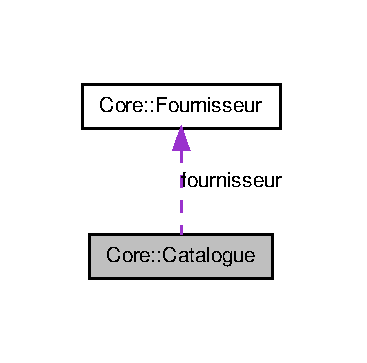
\includegraphics[width=176pt]{de/d4c/class_core_1_1_catalogue__coll__graph}
\end{center}
\end{figure}
\subsection*{Fonctions membres publiques}
\begin{DoxyCompactItemize}
\item 
\hyperlink{class_core_1_1_catalogue_a1563d794f593a4978785d4e784628123}{Catalogue} (QObject $\ast$parent=0)
\begin{DoxyCompactList}\small\item\em Crée un nouveau \hyperlink{class_core_1_1_catalogue}{Catalogue}. \item\end{DoxyCompactList}\item 
\hyperlink{class_core_1_1_catalogue_a56f8f6931050a2592ebc2b2cb3f5ef1d}{Catalogue} (QString code, QObject $\ast$parent=0)
\begin{DoxyCompactList}\small\item\em Crée un nouveau \hyperlink{class_core_1_1_catalogue}{Catalogue}. \item\end{DoxyCompactList}\item 
\hyperlink{class_core_1_1_catalogue_a5a96958fe38e82024175a2dbb40d7d29}{Catalogue} (QString code, QDate dateEnregistrement, QObject $\ast$parent=0)
\begin{DoxyCompactList}\small\item\em Crée un nouveau \hyperlink{class_core_1_1_catalogue}{Catalogue}. \item\end{DoxyCompactList}\item 
QString \hyperlink{class_core_1_1_catalogue_a6dcea2e7862042cd9f05dae894d47a7c}{getCode} () const 
\begin{DoxyCompactList}\small\item\em Renvoie le code du catalogue. \item\end{DoxyCompactList}\item 
QDate \hyperlink{class_core_1_1_catalogue_ac60f6d1630d03598e313ba497ab18f56}{getDateEnregistrement} () const 
\begin{DoxyCompactList}\small\item\em Renvoie la date à laquelle le catalogue a été enregistré \item\end{DoxyCompactList}\item 
\hyperlink{class_core_1_1_fournisseur}{Fournisseur} $\ast$ \hyperlink{class_core_1_1_catalogue_aa8d603a01cab36e2be56a2f10219b56c}{getFournisseur} () const 
\begin{DoxyCompactList}\small\item\em Renvoie l'objet \hyperlink{class_core_1_1_fournisseur}{Fournisseur} correspondant au fournisseur dont émane le catalogue. \item\end{DoxyCompactList}\item 
void \hyperlink{class_core_1_1_catalogue_a065f70f6b69ff02593e0be7813142be4}{setCode} (QString code)
\begin{DoxyCompactList}\small\item\em Modifie le code du catalogue. \item\end{DoxyCompactList}\item 
void \hyperlink{class_core_1_1_catalogue_a722b8c534479e7aad59a7d425250617c}{setDateEnregistrement} (QDate dateEnregistrement)
\begin{DoxyCompactList}\small\item\em Modifie la date d'enregistrement du catalogue. \item\end{DoxyCompactList}\item 
void \hyperlink{class_core_1_1_catalogue_a5f1c6cd886338385a95ce8105dfd48e1}{setFournisseur} (\hyperlink{class_core_1_1_fournisseur}{Fournisseur} $\ast$fournisseur)
\begin{DoxyCompactList}\small\item\em Modifie le fournisseur associé au catalogue. \item\end{DoxyCompactList}\item 
\hypertarget{class_core_1_1_catalogue_a4ec6a17ae60cd156cfb26948a95aeb6e}{
\hyperlink{class_core_1_1_fournisseur}{Fournisseur} $\ast$ {\bfseries getRelation} () const }
\label{de/d33/class_core_1_1_catalogue_a4ec6a17ae60cd156cfb26948a95aeb6e}

\end{DoxyCompactItemize}
\subsection*{Propriétés}
\begin{DoxyCompactItemize}
\item 
\hypertarget{class_core_1_1_catalogue_a8821131af357a9b16ae6b94b4a981eff}{
QString {\bfseries code}}
\label{de/d33/class_core_1_1_catalogue_a8821131af357a9b16ae6b94b4a981eff}

\item 
\hypertarget{class_core_1_1_catalogue_a48107e765325b571457934fbb91eef1b}{
QDate {\bfseries dateEnregistrement}}
\label{de/d33/class_core_1_1_catalogue_a48107e765325b571457934fbb91eef1b}

\item 
\hypertarget{class_core_1_1_catalogue_a39f10786cea1e953b528ef7ba5af054a}{
\hyperlink{class_core_1_1_fournisseur}{Fournisseur} {\bfseries fournisseur}}
\label{de/d33/class_core_1_1_catalogue_a39f10786cea1e953b528ef7ba5af054a}

\end{DoxyCompactItemize}


\subsection{Description détaillée}
Classe représentant un catalogue. \begin{DoxyAuthor}{Auteur}
Pandam, Soumsa, Tchirou, Wouro-\/Sama 
\end{DoxyAuthor}


Définition à la ligne 13 du fichier catalogue.h.



\subsection{Documentation des constructeurs et destructeur}
\hypertarget{class_core_1_1_catalogue_a1563d794f593a4978785d4e784628123}{
\index{Core::Catalogue@{Core::Catalogue}!Catalogue@{Catalogue}}
\index{Catalogue@{Catalogue}!Core::Catalogue@{Core::Catalogue}}
\subsubsection[{Catalogue}]{\setlength{\rightskip}{0pt plus 5cm}Core::Catalogue::Catalogue (
\begin{DoxyParamCaption}
\item[{QObject $\ast$}]{parent = {\ttfamily 0}}
\end{DoxyParamCaption}
)}}
\label{de/d33/class_core_1_1_catalogue_a1563d794f593a4978785d4e784628123}


Crée un nouveau \hyperlink{class_core_1_1_catalogue}{Catalogue}. 


\begin{DoxyParams}{Paramètres}
{\em parent} & Un pointeur vers l'objet parent du \hyperlink{class_core_1_1_catalogue}{Catalogue} \\
\hline
\end{DoxyParams}


Définition à la ligne 12 du fichier catalogue.cpp.

\hypertarget{class_core_1_1_catalogue_a56f8f6931050a2592ebc2b2cb3f5ef1d}{
\index{Core::Catalogue@{Core::Catalogue}!Catalogue@{Catalogue}}
\index{Catalogue@{Catalogue}!Core::Catalogue@{Core::Catalogue}}
\subsubsection[{Catalogue}]{\setlength{\rightskip}{0pt plus 5cm}Core::Catalogue::Catalogue (
\begin{DoxyParamCaption}
\item[{QString}]{code, }
\item[{QObject $\ast$}]{parent = {\ttfamily 0}}
\end{DoxyParamCaption}
)}}
\label{de/d33/class_core_1_1_catalogue_a56f8f6931050a2592ebc2b2cb3f5ef1d}


Crée un nouveau \hyperlink{class_core_1_1_catalogue}{Catalogue}. 


\begin{DoxyParams}{Paramètres}
{\em code} & Le code du \hyperlink{class_core_1_1_catalogue}{Catalogue} \\
\hline
{\em parent} & Un pointeur vers l'objet parent du \hyperlink{class_core_1_1_catalogue}{Catalogue} \\
\hline
\end{DoxyParams}


Définition à la ligne 21 du fichier catalogue.cpp.

\hypertarget{class_core_1_1_catalogue_a5a96958fe38e82024175a2dbb40d7d29}{
\index{Core::Catalogue@{Core::Catalogue}!Catalogue@{Catalogue}}
\index{Catalogue@{Catalogue}!Core::Catalogue@{Core::Catalogue}}
\subsubsection[{Catalogue}]{\setlength{\rightskip}{0pt plus 5cm}Core::Catalogue::Catalogue (
\begin{DoxyParamCaption}
\item[{QString}]{code, }
\item[{QDate}]{dateEnregistrement, }
\item[{QObject $\ast$}]{parent = {\ttfamily 0}}
\end{DoxyParamCaption}
)}}
\label{de/d33/class_core_1_1_catalogue_a5a96958fe38e82024175a2dbb40d7d29}


Crée un nouveau \hyperlink{class_core_1_1_catalogue}{Catalogue}. 


\begin{DoxyParams}{Paramètres}
{\em code} & Le code du \hyperlink{class_core_1_1_catalogue}{Catalogue} \\
\hline
{\em dateEnregistrement} & La date à laquelle le catalogue a été reçu \\
\hline
\end{DoxyParams}


Définition à la ligne 32 du fichier catalogue.cpp.



\subsection{Documentation des fonctions membres}
\hypertarget{class_core_1_1_catalogue_a6dcea2e7862042cd9f05dae894d47a7c}{
\index{Core::Catalogue@{Core::Catalogue}!getCode@{getCode}}
\index{getCode@{getCode}!Core::Catalogue@{Core::Catalogue}}
\subsubsection[{getCode}]{\setlength{\rightskip}{0pt plus 5cm}QString Core::Catalogue::getCode (
\begin{DoxyParamCaption}
{}
\end{DoxyParamCaption}
) const}}
\label{de/d33/class_core_1_1_catalogue_a6dcea2e7862042cd9f05dae894d47a7c}


Renvoie le code du catalogue. 

\begin{DoxyReturn}{Renvoie}
code Le code du catalogue 
\end{DoxyReturn}


Définition à la ligne 43 du fichier catalogue.cpp.

\hypertarget{class_core_1_1_catalogue_ac60f6d1630d03598e313ba497ab18f56}{
\index{Core::Catalogue@{Core::Catalogue}!getDateEnregistrement@{getDateEnregistrement}}
\index{getDateEnregistrement@{getDateEnregistrement}!Core::Catalogue@{Core::Catalogue}}
\subsubsection[{getDateEnregistrement}]{\setlength{\rightskip}{0pt plus 5cm}QDate Core::Catalogue::getDateEnregistrement (
\begin{DoxyParamCaption}
{}
\end{DoxyParamCaption}
) const}}
\label{de/d33/class_core_1_1_catalogue_ac60f6d1630d03598e313ba497ab18f56}


Renvoie la date à laquelle le catalogue a été enregistré 

\begin{DoxyReturn}{Renvoie}
dateEnregistrement La date d'enregistrement du catalogue 
\end{DoxyReturn}


Définition à la ligne 51 du fichier catalogue.cpp.

\hypertarget{class_core_1_1_catalogue_aa8d603a01cab36e2be56a2f10219b56c}{
\index{Core::Catalogue@{Core::Catalogue}!getFournisseur@{getFournisseur}}
\index{getFournisseur@{getFournisseur}!Core::Catalogue@{Core::Catalogue}}
\subsubsection[{getFournisseur}]{\setlength{\rightskip}{0pt plus 5cm}{\bf Fournisseur} $\ast$ Core::Catalogue::getFournisseur (
\begin{DoxyParamCaption}
{}
\end{DoxyParamCaption}
) const}}
\label{de/d33/class_core_1_1_catalogue_aa8d603a01cab36e2be56a2f10219b56c}


Renvoie l'objet \hyperlink{class_core_1_1_fournisseur}{Fournisseur} correspondant au fournisseur dont émane le catalogue. 

\begin{DoxyReturn}{Renvoie}
fournisseur Le fournisseur associé au catalogue 
\end{DoxyReturn}


Définition à la ligne 59 du fichier catalogue.cpp.

\hypertarget{class_core_1_1_catalogue_a065f70f6b69ff02593e0be7813142be4}{
\index{Core::Catalogue@{Core::Catalogue}!setCode@{setCode}}
\index{setCode@{setCode}!Core::Catalogue@{Core::Catalogue}}
\subsubsection[{setCode}]{\setlength{\rightskip}{0pt plus 5cm}void Core::Catalogue::setCode (
\begin{DoxyParamCaption}
\item[{QString}]{code}
\end{DoxyParamCaption}
)}}
\label{de/d33/class_core_1_1_catalogue_a065f70f6b69ff02593e0be7813142be4}


Modifie le code du catalogue. 


\begin{DoxyParams}{Paramètres}
{\em code} & Le nouveau code du catalogue \\
\hline
\end{DoxyParams}


Définition à la ligne 67 du fichier catalogue.cpp.

\hypertarget{class_core_1_1_catalogue_a722b8c534479e7aad59a7d425250617c}{
\index{Core::Catalogue@{Core::Catalogue}!setDateEnregistrement@{setDateEnregistrement}}
\index{setDateEnregistrement@{setDateEnregistrement}!Core::Catalogue@{Core::Catalogue}}
\subsubsection[{setDateEnregistrement}]{\setlength{\rightskip}{0pt plus 5cm}void Core::Catalogue::setDateEnregistrement (
\begin{DoxyParamCaption}
\item[{QDate}]{dateEnregistrement}
\end{DoxyParamCaption}
)}}
\label{de/d33/class_core_1_1_catalogue_a722b8c534479e7aad59a7d425250617c}


Modifie la date d'enregistrement du catalogue. 


\begin{DoxyParams}{Paramètres}
{\em dateEnregistrement} & La nouvelle date d'enregistrement \\
\hline
\end{DoxyParams}


Définition à la ligne 75 du fichier catalogue.cpp.

\hypertarget{class_core_1_1_catalogue_a5f1c6cd886338385a95ce8105dfd48e1}{
\index{Core::Catalogue@{Core::Catalogue}!setFournisseur@{setFournisseur}}
\index{setFournisseur@{setFournisseur}!Core::Catalogue@{Core::Catalogue}}
\subsubsection[{setFournisseur}]{\setlength{\rightskip}{0pt plus 5cm}void Core::Catalogue::setFournisseur (
\begin{DoxyParamCaption}
\item[{{\bf Fournisseur} $\ast$}]{fournisseur}
\end{DoxyParamCaption}
)}}
\label{de/d33/class_core_1_1_catalogue_a5f1c6cd886338385a95ce8105dfd48e1}


Modifie le fournisseur associé au catalogue. 


\begin{DoxyParams}{Paramètres}
{\em fournisseur} & Le fournisseur qui sera associé au catalogue \\
\hline
\end{DoxyParams}


Définition à la ligne 83 du fichier catalogue.cpp.



La documentation de cette classe a été générée à partir des fichiers suivants :\begin{DoxyCompactItemize}
\item 
core/catalogue.h\item 
core/catalogue.cpp\end{DoxyCompactItemize}

\hypertarget{class_core_1_1_centrale_achat}{
\section{Référence de la classe Core::CentraleAchat}
\label{da/d4d/class_core_1_1_centrale_achat}\index{Core::CentraleAchat@{Core::CentraleAchat}}
}


Graphe de collaboration de Core::CentraleAchat:\nopagebreak
\begin{figure}[H]
\begin{center}
\leavevmode
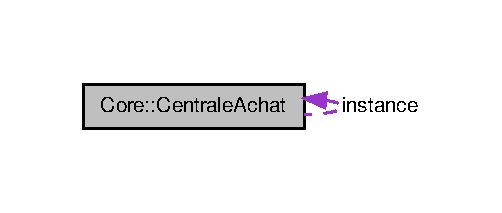
\includegraphics[width=241pt]{df/d06/class_core_1_1_centrale_achat__coll__graph}
\end{center}
\end{figure}
\subsection*{Fonctions membres publiques}
\begin{DoxyCompactItemize}
\item 
\hypertarget{class_core_1_1_centrale_achat_a284b044048a7bd67ad63029ec60fcdcc}{
QString {\bfseries getCode} () const }
\label{da/d4d/class_core_1_1_centrale_achat_a284b044048a7bd67ad63029ec60fcdcc}

\item 
\hypertarget{class_core_1_1_centrale_achat_a899f3f4e45dc3208d2116b600a5b58cd}{
QString {\bfseries getNom} () const }
\label{da/d4d/class_core_1_1_centrale_achat_a899f3f4e45dc3208d2116b600a5b58cd}

\item 
\hypertarget{class_core_1_1_centrale_achat_aa796609a851120d03b7e469b9b380f3b}{
QString {\bfseries getAdresse} () const }
\label{da/d4d/class_core_1_1_centrale_achat_aa796609a851120d03b7e469b9b380f3b}

\item 
\hypertarget{class_core_1_1_centrale_achat_aea0f8c24a1c8438cd86b8ea665e2e812}{
void {\bfseries setCode} (QString code)}
\label{da/d4d/class_core_1_1_centrale_achat_aea0f8c24a1c8438cd86b8ea665e2e812}

\item 
\hypertarget{class_core_1_1_centrale_achat_a6f3a2d24f3669d7d5accb8f14a5ece2d}{
void {\bfseries setNom} (QString nom)}
\label{da/d4d/class_core_1_1_centrale_achat_a6f3a2d24f3669d7d5accb8f14a5ece2d}

\item 
\hypertarget{class_core_1_1_centrale_achat_a6affd660ba7fd08e4decc45aaafde5d1}{
void {\bfseries setAdresse} (QString adresse)}
\label{da/d4d/class_core_1_1_centrale_achat_a6affd660ba7fd08e4decc45aaafde5d1}

\item 
\hypertarget{class_core_1_1_centrale_achat_aa48c7e26bc294f8c0255e39ab40860ea}{
bool {\bfseries save} ()}
\label{da/d4d/class_core_1_1_centrale_achat_aa48c7e26bc294f8c0255e39ab40860ea}

\end{DoxyCompactItemize}
\subsection*{Fonctions membres publiques statiques}
\begin{DoxyCompactItemize}
\item 
\hypertarget{class_core_1_1_centrale_achat_a847763b5f69932f81a29335e32028a6b}{
static \hyperlink{class_core_1_1_centrale_achat}{CentraleAchat} $\ast$ {\bfseries getInstance} ()}
\label{da/d4d/class_core_1_1_centrale_achat_a847763b5f69932f81a29335e32028a6b}

\end{DoxyCompactItemize}


\subsection{Description détaillée}


Définition à la ligne 8 du fichier centraleachat.h.



La documentation de cette classe a été générée à partir des fichiers suivants :\begin{DoxyCompactItemize}
\item 
core/centraleachat.h\item 
core/centraleachat.cpp\end{DoxyCompactItemize}

\hypertarget{class_core_1_1_commande}{
\section{Référence de la classe Core::Commande}
\label{d0/d92/class_core_1_1_commande}\index{Core::Commande@{Core::Commande}}
}


Graphe de collaboration de Core::Commande:\nopagebreak
\begin{figure}[H]
\begin{center}
\leavevmode
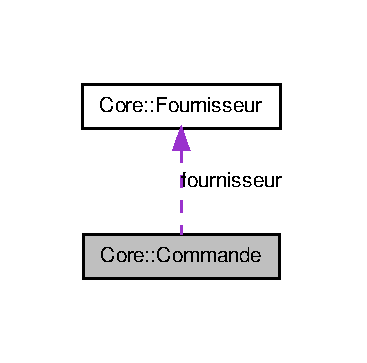
\includegraphics[width=176pt]{d4/da3/class_core_1_1_commande__coll__graph}
\end{center}
\end{figure}
\subsection*{Types publics}
\begin{DoxyCompactItemize}
\item 
enum {\bfseries Etat} \{ {\bfseries EnAttente}, 
{\bfseries EnAttenteLivraison}, 
{\bfseries LivraisonPartielle}, 
{\bfseries LivraisonTotale}
 \}
\end{DoxyCompactItemize}
\subsection*{Fonctions membres publiques}
\begin{DoxyCompactItemize}
\item 
\hypertarget{class_core_1_1_commande_a64cb1834d666c1ec9f6cb0f11b5f9c78}{
{\bfseries Commande} (QObject $\ast$parent=0)}
\label{d0/d92/class_core_1_1_commande_a64cb1834d666c1ec9f6cb0f11b5f9c78}

\item 
\hypertarget{class_core_1_1_commande_ad24bf970d58e268642a102650698ba6e}{
{\bfseries Commande} (QString code, QObject $\ast$parent=0)}
\label{d0/d92/class_core_1_1_commande_ad24bf970d58e268642a102650698ba6e}

\item 
\hypertarget{class_core_1_1_commande_ad9219981f0c67b8627924c422c968aa6}{
{\bfseries Commande} (QString code, QDate date, QObject $\ast$parent=0)}
\label{d0/d92/class_core_1_1_commande_ad9219981f0c67b8627924c422c968aa6}

\item 
\hypertarget{class_core_1_1_commande_af17d69972864c85cf980845772bc737f}{
QString {\bfseries getCode} () const }
\label{d0/d92/class_core_1_1_commande_af17d69972864c85cf980845772bc737f}

\item 
\hypertarget{class_core_1_1_commande_a89b8b550e9eeea14e5c7c81e06bf485a}{
QDate {\bfseries getDate} () const }
\label{d0/d92/class_core_1_1_commande_a89b8b550e9eeea14e5c7c81e06bf485a}

\item 
\hypertarget{class_core_1_1_commande_a3d2b4980b3472ac81e91be956a6ac537}{
int {\bfseries getEtat} () const }
\label{d0/d92/class_core_1_1_commande_a3d2b4980b3472ac81e91be956a6ac537}

\item 
\hypertarget{class_core_1_1_commande_a8b86b2723f049285eef734c72585e704}{
\hyperlink{class_core_1_1_fournisseur}{Fournisseur} $\ast$ {\bfseries getFournisseur} () const }
\label{d0/d92/class_core_1_1_commande_a8b86b2723f049285eef734c72585e704}

\item 
\hypertarget{class_core_1_1_commande_a81e784a1aedef144d76642d318b74b71}{
void {\bfseries setCode} (QString code)}
\label{d0/d92/class_core_1_1_commande_a81e784a1aedef144d76642d318b74b71}

\item 
\hypertarget{class_core_1_1_commande_af031ef6f31adc61a5f3377eda393de75}{
void {\bfseries setDate} (QDate date)}
\label{d0/d92/class_core_1_1_commande_af031ef6f31adc61a5f3377eda393de75}

\item 
\hypertarget{class_core_1_1_commande_af52344f6b446455c79ab3a6e9cb9b88e}{
void {\bfseries setEtat} (int etat)}
\label{d0/d92/class_core_1_1_commande_af52344f6b446455c79ab3a6e9cb9b88e}

\item 
\hypertarget{class_core_1_1_commande_a92c4d0da3e627176e5899154d8cd73f8}{
void {\bfseries setFournisseur} (\hyperlink{class_core_1_1_fournisseur}{Fournisseur} $\ast$fournisseur)}
\label{d0/d92/class_core_1_1_commande_a92c4d0da3e627176e5899154d8cd73f8}

\item 
\hypertarget{class_core_1_1_commande_a9788565cf3467dd64869b684a92ef096}{
\hyperlink{class_core_1_1_fournisseur}{Fournisseur} $\ast$ {\bfseries getRelation} () const }
\label{d0/d92/class_core_1_1_commande_a9788565cf3467dd64869b684a92ef096}

\end{DoxyCompactItemize}
\subsection*{Propriétés}
\begin{DoxyCompactItemize}
\item 
\hypertarget{class_core_1_1_commande_af012ec6904b174e6487c279989c3e622}{
QString {\bfseries code}}
\label{d0/d92/class_core_1_1_commande_af012ec6904b174e6487c279989c3e622}

\item 
\hypertarget{class_core_1_1_commande_a18973533ff7bddd4dd2bc047cc93a738}{
QDate {\bfseries date}}
\label{d0/d92/class_core_1_1_commande_a18973533ff7bddd4dd2bc047cc93a738}

\item 
\hypertarget{class_core_1_1_commande_a6db42c7e148b1ef83a3d2988814dc547}{
int {\bfseries etat}}
\label{d0/d92/class_core_1_1_commande_a6db42c7e148b1ef83a3d2988814dc547}

\item 
\hypertarget{class_core_1_1_commande_a1f6d336f1eab3a0471ddea678d106e00}{
\hyperlink{class_core_1_1_fournisseur}{Fournisseur} {\bfseries fournisseur}}
\label{d0/d92/class_core_1_1_commande_a1f6d336f1eab3a0471ddea678d106e00}

\end{DoxyCompactItemize}


\subsection{Description détaillée}


Définition à la ligne 9 du fichier commande.h.



La documentation de cette classe a été générée à partir des fichiers suivants :\begin{DoxyCompactItemize}
\item 
core/commande.h\item 
core/commande.cpp\end{DoxyCompactItemize}

\hypertarget{class_core_1_1_connection}{
\section{Référence de la classe Core::Connection}
\label{d9/de1/class_core_1_1_connection}\index{Core::Connection@{Core::Connection}}
}


Graphe de collaboration de Core::Connection:\nopagebreak
\begin{figure}[H]
\begin{center}
\leavevmode
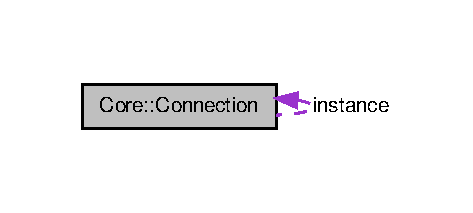
\includegraphics[width=227pt]{d3/d0c/class_core_1_1_connection__coll__graph}
\end{center}
\end{figure}
\subsection*{Fonctions membres publiques}
\begin{DoxyCompactItemize}
\item 
\hypertarget{class_core_1_1_connection_afdc9348dddce61b32603392b0184afd2}{
bool {\bfseries connecter} ()}
\label{d9/de1/class_core_1_1_connection_afdc9348dddce61b32603392b0184afd2}

\item 
\hypertarget{class_core_1_1_connection_a7c6a447d9dc62697749967243076c050}{
void {\bfseries creerTablesSingletons} ()}
\label{d9/de1/class_core_1_1_connection_a7c6a447d9dc62697749967243076c050}

\end{DoxyCompactItemize}
\subsection*{Fonctions membres publiques statiques}
\begin{DoxyCompactItemize}
\item 
\hypertarget{class_core_1_1_connection_ae13db59cd64ea83af1f344cfab170fd1}{
static \hyperlink{class_core_1_1_connection}{Connection} $\ast$ {\bfseries getInstance} ()}
\label{d9/de1/class_core_1_1_connection_ae13db59cd64ea83af1f344cfab170fd1}

\end{DoxyCompactItemize}


\subsection{Description détaillée}


Définition à la ligne 29 du fichier connection.h.



La documentation de cette classe a été générée à partir des fichiers suivants :\begin{DoxyCompactItemize}
\item 
core/connection.h\item 
core/connection.cpp\end{DoxyCompactItemize}

\hypertarget{class_core_1_1_fournisseur}{
\section{Référence de la classe Core::Fournisseur}
\label{dd/d46/class_core_1_1_fournisseur}\index{Core::Fournisseur@{Core::Fournisseur}}
}
\subsection*{Fonctions membres publiques}
\begin{DoxyCompactItemize}
\item 
\hypertarget{class_core_1_1_fournisseur_a92a66f86c739e9d99e706f37e20c9e23}{
{\bfseries Fournisseur} (QObject $\ast$parent=0)}
\label{dd/d46/class_core_1_1_fournisseur_a92a66f86c739e9d99e706f37e20c9e23}

\item 
\hypertarget{class_core_1_1_fournisseur_aa1769c68daafe9ca019e7f44b58733ab}{
{\bfseries Fournisseur} (QString code, QObject $\ast$parent=0)}
\label{dd/d46/class_core_1_1_fournisseur_aa1769c68daafe9ca019e7f44b58733ab}

\item 
\hypertarget{class_core_1_1_fournisseur_a589b320b955a1d579289feb1a86b1b1a}{
{\bfseries Fournisseur} (QString code, QString nom, QString adresse, QObject $\ast$parent=0)}
\label{dd/d46/class_core_1_1_fournisseur_a589b320b955a1d579289feb1a86b1b1a}

\item 
\hypertarget{class_core_1_1_fournisseur_a2057eff46212798f46a77f796843a85b}{
QString {\bfseries getCode} () const }
\label{dd/d46/class_core_1_1_fournisseur_a2057eff46212798f46a77f796843a85b}

\item 
\hypertarget{class_core_1_1_fournisseur_a1992269f4001ee5334da232cd38b0b4f}{
QString {\bfseries getNom} () const }
\label{dd/d46/class_core_1_1_fournisseur_a1992269f4001ee5334da232cd38b0b4f}

\item 
\hypertarget{class_core_1_1_fournisseur_a72dad10866538b2d8b85a89cfd913120}{
QString {\bfseries getAdresse} () const }
\label{dd/d46/class_core_1_1_fournisseur_a72dad10866538b2d8b85a89cfd913120}

\item 
\hypertarget{class_core_1_1_fournisseur_adf1f53ad62c589fd3d899b80df8f4aba}{
void {\bfseries setCode} (QString code)}
\label{dd/d46/class_core_1_1_fournisseur_adf1f53ad62c589fd3d899b80df8f4aba}

\item 
\hypertarget{class_core_1_1_fournisseur_a28c8cef8779014374039af0995a12153}{
void {\bfseries setNom} (QString nom)}
\label{dd/d46/class_core_1_1_fournisseur_a28c8cef8779014374039af0995a12153}

\item 
\hypertarget{class_core_1_1_fournisseur_a9749cce0ebc40fd3a3791490cea9bb9c}{
void {\bfseries setAdresse} (QString adresse)}
\label{dd/d46/class_core_1_1_fournisseur_a9749cce0ebc40fd3a3791490cea9bb9c}

\end{DoxyCompactItemize}
\subsection*{Propriétés}
\begin{DoxyCompactItemize}
\item 
\hypertarget{class_core_1_1_fournisseur_a02dffbeb8baad2a751853224906eb368}{
QString {\bfseries code}}
\label{dd/d46/class_core_1_1_fournisseur_a02dffbeb8baad2a751853224906eb368}

\item 
\hypertarget{class_core_1_1_fournisseur_a13a6cff7c601b36e547fc753cfd96b9e}{
QString {\bfseries nom}}
\label{dd/d46/class_core_1_1_fournisseur_a13a6cff7c601b36e547fc753cfd96b9e}

\item 
\hypertarget{class_core_1_1_fournisseur_a6f897b77982a6b9fae7e76a04cf4ea9e}{
QString {\bfseries adresse}}
\label{dd/d46/class_core_1_1_fournisseur_a6f897b77982a6b9fae7e76a04cf4ea9e}

\end{DoxyCompactItemize}


\subsection{Description détaillée}


Définition à la ligne 8 du fichier fournisseur.h.



La documentation de cette classe a été générée à partir des fichiers suivants :\begin{DoxyCompactItemize}
\item 
core/fournisseur.h\item 
core/fournisseur.cpp\end{DoxyCompactItemize}

\hypertarget{class_imprimante}{
\section{Imprimante Class Reference}
\label{class_imprimante}\index{Imprimante@{Imprimante}}
}


\subsection{Detailed Description}


Definition at line 4 of file imprimante.h.



The documentation for this class was generated from the following files:\begin{DoxyCompactItemize}
\item 
core/imprimante.h\item 
core/imprimante.cpp\end{DoxyCompactItemize}

\hypertarget{class_core_1_1_inventaire}{
\section{Référence de la classe Core::Inventaire}
\label{da/d65/class_core_1_1_inventaire}\index{Core::Inventaire@{Core::Inventaire}}
}
\subsection*{Fonctions membres publiques}
\begin{DoxyCompactItemize}
\item 
\hypertarget{class_core_1_1_inventaire_ad01d4ffb33bad2ad7d21bfed4d7663ae}{
{\bfseries Inventaire} (QObject $\ast$parent=0)}
\label{da/d65/class_core_1_1_inventaire_ad01d4ffb33bad2ad7d21bfed4d7663ae}

\item 
\hypertarget{class_core_1_1_inventaire_afd5bb3033dc973009a155766df11dae5}{
{\bfseries Inventaire} (QString code, QObject $\ast$parent=0)}
\label{da/d65/class_core_1_1_inventaire_afd5bb3033dc973009a155766df11dae5}

\item 
\hypertarget{class_core_1_1_inventaire_a6c6a244b43135939b5982d2035335356}{
{\bfseries Inventaire} (QString code, QString nom, QDate date, QObject $\ast$parent=0)}
\label{da/d65/class_core_1_1_inventaire_a6c6a244b43135939b5982d2035335356}

\item 
\hypertarget{class_core_1_1_inventaire_a659e26afcdfc8e05ec3721e51c08807a}{
QString {\bfseries getCode} () const }
\label{da/d65/class_core_1_1_inventaire_a659e26afcdfc8e05ec3721e51c08807a}

\item 
\hypertarget{class_core_1_1_inventaire_a0fe45e53a18447ad719f5cc4925d198c}{
QString {\bfseries getNom} () const }
\label{da/d65/class_core_1_1_inventaire_a0fe45e53a18447ad719f5cc4925d198c}

\item 
\hypertarget{class_core_1_1_inventaire_a2528c5363e7132f6e267a12180795eae}{
QDate {\bfseries getDate} () const }
\label{da/d65/class_core_1_1_inventaire_a2528c5363e7132f6e267a12180795eae}

\item 
\hypertarget{class_core_1_1_inventaire_a26a0a69fa35afbb38e677c431941c95a}{
void {\bfseries setCode} (QString code)}
\label{da/d65/class_core_1_1_inventaire_a26a0a69fa35afbb38e677c431941c95a}

\item 
\hypertarget{class_core_1_1_inventaire_ae667fc03cd096433878fe25947344d12}{
void {\bfseries setNom} (QString nom)}
\label{da/d65/class_core_1_1_inventaire_ae667fc03cd096433878fe25947344d12}

\item 
\hypertarget{class_core_1_1_inventaire_a4e43ba68f958ac2435938eb033e71583}{
void {\bfseries setDate} (QDate date)}
\label{da/d65/class_core_1_1_inventaire_a4e43ba68f958ac2435938eb033e71583}

\end{DoxyCompactItemize}
\subsection*{Propriétés}
\begin{DoxyCompactItemize}
\item 
\hypertarget{class_core_1_1_inventaire_a779e2eca216bb9db2a47bfdf909d53c6}{
QString {\bfseries code}}
\label{da/d65/class_core_1_1_inventaire_a779e2eca216bb9db2a47bfdf909d53c6}

\item 
\hypertarget{class_core_1_1_inventaire_af293861f1301ffe838d0d018e3398579}{
QString {\bfseries nom}}
\label{da/d65/class_core_1_1_inventaire_af293861f1301ffe838d0d018e3398579}

\item 
\hypertarget{class_core_1_1_inventaire_afa6bc9c32828feb9979f802d7f00b3da}{
QDate {\bfseries date}}
\label{da/d65/class_core_1_1_inventaire_afa6bc9c32828feb9979f802d7f00b3da}

\end{DoxyCompactItemize}


\subsection{Description détaillée}


Définition à la ligne 8 du fichier inventaire.h.



La documentation de cette classe a été générée à partir des fichiers suivants :\begin{DoxyCompactItemize}
\item 
core/inventaire.h\item 
core/inventaire.cpp\end{DoxyCompactItemize}

\hypertarget{class_core_1_1_livraison}{
\section{Référence de la classe Core::Livraison}
\label{df/d27/class_core_1_1_livraison}\index{Core::Livraison@{Core::Livraison}}
}


Graphe de collaboration de Core::Livraison:\nopagebreak
\begin{figure}[H]
\begin{center}
\leavevmode
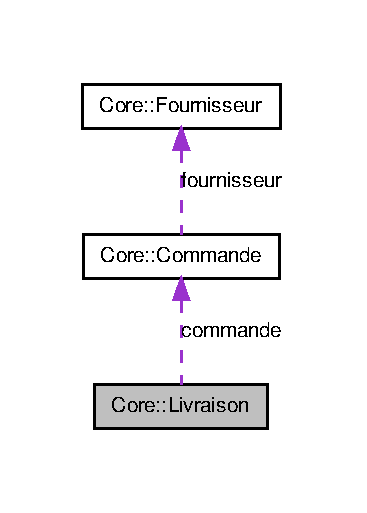
\includegraphics[width=176pt]{db/def/class_core_1_1_livraison__coll__graph}
\end{center}
\end{figure}
\subsection*{Fonctions membres publiques}
\begin{DoxyCompactItemize}
\item 
\hypertarget{class_core_1_1_livraison_aa379bd1af2efc8ec306d6c67ee8f4261}{
{\bfseries Livraison} (QObject $\ast$parent=0)}
\label{df/d27/class_core_1_1_livraison_aa379bd1af2efc8ec306d6c67ee8f4261}

\item 
\hypertarget{class_core_1_1_livraison_a80b3e82dc3309a7a62fb3c49d13d9192}{
{\bfseries Livraison} (QString code, QObject $\ast$parent=0)}
\label{df/d27/class_core_1_1_livraison_a80b3e82dc3309a7a62fb3c49d13d9192}

\item 
\hypertarget{class_core_1_1_livraison_ad05b42ede2806b27073c8838832a07d6}{
{\bfseries Livraison} (QString code, QDate date, QObject $\ast$parent=0)}
\label{df/d27/class_core_1_1_livraison_ad05b42ede2806b27073c8838832a07d6}

\item 
\hypertarget{class_core_1_1_livraison_a94c4cb5ef6f414eea4efcad5e28b9eb0}{
QString {\bfseries getCode} () const }
\label{df/d27/class_core_1_1_livraison_a94c4cb5ef6f414eea4efcad5e28b9eb0}

\item 
\hypertarget{class_core_1_1_livraison_a1a804da6b7b0ab0e35cab544fdbe98c6}{
QDate {\bfseries getDate} () const }
\label{df/d27/class_core_1_1_livraison_a1a804da6b7b0ab0e35cab544fdbe98c6}

\item 
\hypertarget{class_core_1_1_livraison_aeb7fc3228969963e1ee963b8f3c5fd68}{
\hyperlink{class_core_1_1_commande}{Commande} $\ast$ {\bfseries getCommande} () const }
\label{df/d27/class_core_1_1_livraison_aeb7fc3228969963e1ee963b8f3c5fd68}

\item 
\hypertarget{class_core_1_1_livraison_acadeeaa69380464672ca9d570b69dc68}{
void {\bfseries setCode} (QString code)}
\label{df/d27/class_core_1_1_livraison_acadeeaa69380464672ca9d570b69dc68}

\item 
\hypertarget{class_core_1_1_livraison_ad556ab227f0a8b89065a6158384fc6f2}{
void {\bfseries setDate} (QDate date)}
\label{df/d27/class_core_1_1_livraison_ad556ab227f0a8b89065a6158384fc6f2}

\item 
\hypertarget{class_core_1_1_livraison_a300de117ed9872251c4b3a02183db114}{
void {\bfseries setCommande} (\hyperlink{class_core_1_1_commande}{Commande} $\ast$commande)}
\label{df/d27/class_core_1_1_livraison_a300de117ed9872251c4b3a02183db114}

\item 
\hypertarget{class_core_1_1_livraison_a8757eceef21d0f3edc13e2c2c11b651e}{
\hyperlink{class_core_1_1_commande}{Commande} $\ast$ {\bfseries getRelation} () const }
\label{df/d27/class_core_1_1_livraison_a8757eceef21d0f3edc13e2c2c11b651e}

\end{DoxyCompactItemize}
\subsection*{Propriétés}
\begin{DoxyCompactItemize}
\item 
\hypertarget{class_core_1_1_livraison_a05faa701617f0d602f3c3ecdcfebba9d}{
QString {\bfseries code}}
\label{df/d27/class_core_1_1_livraison_a05faa701617f0d602f3c3ecdcfebba9d}

\item 
\hypertarget{class_core_1_1_livraison_a0ecb446fad5ddf4f46c079a6b1dea5be}{
QDate {\bfseries date}}
\label{df/d27/class_core_1_1_livraison_a0ecb446fad5ddf4f46c079a6b1dea5be}

\item 
\hypertarget{class_core_1_1_livraison_a29e340b05d4914fa9bff496219e932ac}{
\hyperlink{class_core_1_1_commande}{Commande} {\bfseries commande}}
\label{df/d27/class_core_1_1_livraison_a29e340b05d4914fa9bff496219e932ac}

\end{DoxyCompactItemize}


\subsection{Description détaillée}


Définition à la ligne 8 du fichier livraison.h.



La documentation de cette classe a été générée à partir des fichiers suivants :\begin{DoxyCompactItemize}
\item 
core/livraison.h\item 
core/livraison.cpp\end{DoxyCompactItemize}

\hypertarget{class_logiciel}{
\section{Logiciel Class Reference}
\label{class_logiciel}\index{Logiciel@{Logiciel}}
}


\subsection{Detailed Description}


Definition at line 4 of file logiciel.h.



The documentation for this class was generated from the following files:\begin{DoxyCompactItemize}
\item 
core/logiciel.h\item 
core/logiciel.cpp\end{DoxyCompactItemize}

\hypertarget{class_core_1_1_magasin}{
\section{Référence de la classe Core::Magasin}
\label{db/d58/class_core_1_1_magasin}\index{Core::Magasin@{Core::Magasin}}
}


Graphe de collaboration de Core::Magasin:\nopagebreak
\begin{figure}[H]
\begin{center}
\leavevmode
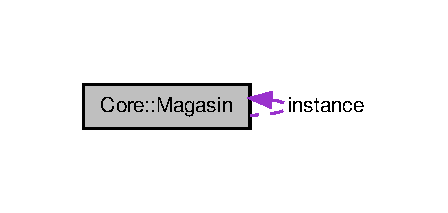
\includegraphics[width=215pt]{dd/dd9/class_core_1_1_magasin__coll__graph}
\end{center}
\end{figure}
\subsection*{Fonctions membres publiques}
\begin{DoxyCompactItemize}
\item 
\hypertarget{class_core_1_1_magasin_a32b4c2ed780a53546f58adf1223a4ab2}{
QString {\bfseries getCode} () const }
\label{db/d58/class_core_1_1_magasin_a32b4c2ed780a53546f58adf1223a4ab2}

\item 
\hypertarget{class_core_1_1_magasin_a4a1c4c2061338b1e612f5ea5cf0f3078}{
QString {\bfseries getNom} () const }
\label{db/d58/class_core_1_1_magasin_a4a1c4c2061338b1e612f5ea5cf0f3078}

\item 
\hypertarget{class_core_1_1_magasin_a4fb857ff7d3a402cc979544fcfbdea2a}{
QString {\bfseries getAdresse} () const }
\label{db/d58/class_core_1_1_magasin_a4fb857ff7d3a402cc979544fcfbdea2a}

\item 
\hypertarget{class_core_1_1_magasin_a9008fda6fea2f34438477ff902ce0e58}{
void {\bfseries setCode} (QString code)}
\label{db/d58/class_core_1_1_magasin_a9008fda6fea2f34438477ff902ce0e58}

\item 
\hypertarget{class_core_1_1_magasin_a6b068992df353cb27b0230f9c6be4392}{
void {\bfseries setNom} (QString nom)}
\label{db/d58/class_core_1_1_magasin_a6b068992df353cb27b0230f9c6be4392}

\item 
\hypertarget{class_core_1_1_magasin_a51aff2a2720390d4dc68061df538a7bf}{
void {\bfseries setAdresse} (QString description)}
\label{db/d58/class_core_1_1_magasin_a51aff2a2720390d4dc68061df538a7bf}

\item 
\hypertarget{class_core_1_1_magasin_a20392ad98fbb23f6b9840b92f7613013}{
bool {\bfseries save} ()}
\label{db/d58/class_core_1_1_magasin_a20392ad98fbb23f6b9840b92f7613013}

\end{DoxyCompactItemize}
\subsection*{Fonctions membres publiques statiques}
\begin{DoxyCompactItemize}
\item 
\hypertarget{class_core_1_1_magasin_a1a9f32f9d91cf3e41d96cabb87593940}{
static \hyperlink{class_core_1_1_magasin}{Magasin} $\ast$ {\bfseries getInstance} ()}
\label{db/d58/class_core_1_1_magasin_a1a9f32f9d91cf3e41d96cabb87593940}

\end{DoxyCompactItemize}


\subsection{Description détaillée}


Définition à la ligne 8 du fichier magasin.h.



La documentation de cette classe a été générée à partir des fichiers suivants :\begin{DoxyCompactItemize}
\item 
core/magasin.h\item 
core/magasin.cpp\end{DoxyCompactItemize}

\hypertarget{class_model_1_1_m_s_relational_table_model}{
\section{Référence de la classe Model::MSRelationalTableModel$<$ S, T $>$ (modèle)}
\label{dc/d52/class_model_1_1_m_s_relational_table_model}\index{Model::MSRelationalTableModel@{Model::MSRelationalTableModel}}
}
\subsection*{Fonctions membres publiques}
\begin{DoxyCompactItemize}
\item 
\hypertarget{class_model_1_1_m_s_relational_table_model_a4edf02555589b8ab37b0aa8e40a9a92c}{
{\bfseries MSRelationalTableModel} (QObject $\ast$parent=0)}
\label{dc/d52/class_model_1_1_m_s_relational_table_model_a4edf02555589b8ab37b0aa8e40a9a92c}

\item 
\hypertarget{class_model_1_1_m_s_relational_table_model_a64c0a17b9dfd48271cd0c4935c999a74}{
{\bfseries MSRelationalTableModel} (const QDjangoQuerySet$<$ S $>$ \&source, const QDjangoQuerySet$<$ T $>$ \&cible, QObject $\ast$parent=0)}
\label{dc/d52/class_model_1_1_m_s_relational_table_model_a64c0a17b9dfd48271cd0c4935c999a74}

\item 
\hypertarget{class_model_1_1_m_s_relational_table_model_ac8ff373f4ade27feb5983132705082b7}{
{\bfseries MSRelationalTableModel} (const QDjangoQuerySet$<$ S $>$ \&source, const QDjangoQuerySet$<$ T $>$ \&cible, const char $\ast$liaison, QObject $\ast$parent=0)}
\label{dc/d52/class_model_1_1_m_s_relational_table_model_ac8ff373f4ade27feb5983132705082b7}

\item 
\hypertarget{class_model_1_1_m_s_relational_table_model_a62f7a5c786ba2c13c7bf5769243d0526}{
void {\bfseries setSrcQuerySet} (QDjangoQuerySet$<$ S $>$ \&source)}
\label{dc/d52/class_model_1_1_m_s_relational_table_model_a62f7a5c786ba2c13c7bf5769243d0526}

\item 
\hypertarget{class_model_1_1_m_s_relational_table_model_a5cb2019d998ae621124417af3825404d}{
void {\bfseries setDestQuerySet} (QDjangoQuerySet$<$ T $>$ \&cible)}
\label{dc/d52/class_model_1_1_m_s_relational_table_model_a5cb2019d998ae621124417af3825404d}

\item 
\hypertarget{class_model_1_1_m_s_relational_table_model_a4bef4ba16a9f5259dc57f0abb044adf2}{
void {\bfseries setRelation} (const char $\ast$liaison)}
\label{dc/d52/class_model_1_1_m_s_relational_table_model_a4bef4ba16a9f5259dc57f0abb044adf2}

\item 
\hypertarget{class_model_1_1_m_s_relational_table_model_aea32363f52756c4994b6b3f36d20aeeb}{
int {\bfseries rowCount} (const QModelIndex \&parent=QModelIndex()) const }
\label{dc/d52/class_model_1_1_m_s_relational_table_model_aea32363f52756c4994b6b3f36d20aeeb}

\item 
\hypertarget{class_model_1_1_m_s_relational_table_model_a5c6697b029ea56da41a75cb85efa8dfa}{
int {\bfseries columnCount} (const QModelIndex \&parent=QModelIndex()) const }
\label{dc/d52/class_model_1_1_m_s_relational_table_model_a5c6697b029ea56da41a75cb85efa8dfa}

\item 
\hypertarget{class_model_1_1_m_s_relational_table_model_abfa820b5069fd8518e916395103b3d8d}{
QVariant {\bfseries data} (const QModelIndex \&index, int role=Qt::DisplayRole) const }
\label{dc/d52/class_model_1_1_m_s_relational_table_model_abfa820b5069fd8518e916395103b3d8d}

\item 
\hypertarget{class_model_1_1_m_s_relational_table_model_afe6d20c15871c4e6975010744e62994f}{
QVariant {\bfseries headerData} (int section, Qt::Orientation orientation, int role=Qt::DisplayRole) const }
\label{dc/d52/class_model_1_1_m_s_relational_table_model_afe6d20c15871c4e6975010744e62994f}

\end{DoxyCompactItemize}
\subsection*{Attributs publics statiques}
\begin{DoxyCompactItemize}
\item 
\hypertarget{class_model_1_1_m_s_relational_table_model_ad678554e1d2597c4c9e8e04f7893fa9c}{
static const int {\bfseries NB\_\-CHAMPS\_\-PAR\_\-DEFAUT} = 2}
\label{dc/d52/class_model_1_1_m_s_relational_table_model_ad678554e1d2597c4c9e8e04f7893fa9c}

\end{DoxyCompactItemize}


\subsection{Description détaillée}
\subsubsection*{template$<$typename S, typename T$>$ class Model::MSRelationalTableModel$<$ S, T $>$}



Définition à la ligne 14 du fichier msrelationaltablemodel.h.



La documentation de cette classe a été générée à partir du fichier suivant :\begin{DoxyCompactItemize}
\item 
model/msrelationaltablemodel.h\end{DoxyCompactItemize}

\hypertarget{class_model_1_1_m_s_table_model}{
\section{Référence de la classe Model::MSTableModel$<$ S $>$ (modèle)}
\label{dd/df1/class_model_1_1_m_s_table_model}\index{Model::MSTableModel@{Model::MSTableModel}}
}


Classe représentant un modèle dérivant de QAbstractTableModel.  




{\ttfamily \#include $<$mstablemodel.h$>$}

\subsection*{Fonctions membres publiques}
\begin{DoxyCompactItemize}
\item 
\hyperlink{class_model_1_1_m_s_table_model_a30e231f29210374f874984eeb6e0747b}{MSTableModel} (QObject $\ast$parent=0)
\begin{DoxyCompactList}\small\item\em Crée un nouveau \hyperlink{class_model_1_1_m_s_table_model}{MSTableModel}. \item\end{DoxyCompactList}\item 
\hyperlink{class_model_1_1_m_s_table_model_aa33f0d847cdd4bcdf2a3733b1bf74a74}{MSTableModel} (const QDjangoQuerySet$<$ S $>$ \&table, QObject $\ast$parent=0)
\begin{DoxyCompactList}\small\item\em Crée un nouveau \hyperlink{class_model_1_1_m_s_table_model}{MSTableModel}. \item\end{DoxyCompactList}\item 
void \hyperlink{class_model_1_1_m_s_table_model_abde72a77c23d0a8dd452c7e8fe67bb37}{setQuerySet} (QDjangoQuerySet$<$ S $>$ \&table)
\begin{DoxyCompactList}\small\item\em Modifie le QDjangoQuerySet associé au modèle. \item\end{DoxyCompactList}\item 
int \hyperlink{class_model_1_1_m_s_table_model_afed4398e4a30645b9105683ff4f5ee80}{rowCount} (const QModelIndex \&parent=QModelIndex()) const 
\begin{DoxyCompactList}\small\item\em Méthode virtuelle de la classe QAbstractTableModel redéfinie ici pour donner le nombre de lignes du modèle. \item\end{DoxyCompactList}\item 
int \hyperlink{class_model_1_1_m_s_table_model_a1596316183a5ace9d74199da67d49ba5}{columnCount} (const QModelIndex \&parent=QModelIndex()) const 
\begin{DoxyCompactList}\small\item\em Méthode virtuelle de la classe QAbstractTableModel redéfinie qui donne le nombre de colonnes du modèle. \item\end{DoxyCompactList}\item 
QVariant \hyperlink{class_model_1_1_m_s_table_model_ac32ed05114cd690b6b01bd0e4125c3dd}{data} (const QModelIndex \&index, int role=Qt::DisplayRole) const 
\begin{DoxyCompactList}\small\item\em Renvoie la donnée située à une ligne et une colonne précise du modèle. Le numero de ligne est représenté par index.row() et le numero de colonne par index.column() \item\end{DoxyCompactList}\item 
QVariant \hyperlink{class_model_1_1_m_s_table_model_a381ab9cc46824ee8073e6a2989c1a314}{headerData} (int section, Qt::Orientation orientation, int role=Qt::DisplayRole) const 
\begin{DoxyCompactList}\small\item\em Renvoie la chaîne de caractères qui sera affichée en entête de la table à une section donnée. \item\end{DoxyCompactList}\end{DoxyCompactItemize}
\subsection*{Attributs publics statiques}
\begin{DoxyCompactItemize}
\item 
\hypertarget{class_model_1_1_m_s_table_model_aaa19a5fe7e969dcd93024d59ab912ceb}{
static const int {\bfseries NB\_\-CHAMPS\_\-PAR\_\-DEFAUT} = 2}
\label{dd/df1/class_model_1_1_m_s_table_model_aaa19a5fe7e969dcd93024d59ab912ceb}

\end{DoxyCompactItemize}


\subsection{Description détaillée}
\subsubsection*{template$<$typename S$>$ class Model::MSTableModel$<$ S $>$}

Classe représentant un modèle dérivant de QAbstractTableModel. 

Définition à la ligne 20 du fichier mstablemodel.h.



\subsection{Documentation des constructeurs et destructeur}
\hypertarget{class_model_1_1_m_s_table_model_a30e231f29210374f874984eeb6e0747b}{
\index{Model::MSTableModel@{Model::MSTableModel}!MSTableModel@{MSTableModel}}
\index{MSTableModel@{MSTableModel}!Model::MSTableModel@{Model::MSTableModel}}
\subsubsection[{MSTableModel}]{\setlength{\rightskip}{0pt plus 5cm}template$<$typename S $>$ {\bf Model::MSTableModel}$<$ S $>$::{\bf MSTableModel} (
\begin{DoxyParamCaption}
\item[{QObject $\ast$}]{parent = {\ttfamily 0}}
\end{DoxyParamCaption}
)}}
\label{dd/df1/class_model_1_1_m_s_table_model_a30e231f29210374f874984eeb6e0747b}


Crée un nouveau \hyperlink{class_model_1_1_m_s_table_model}{MSTableModel}. 


\begin{DoxyParams}{Paramètres}
{\em parent} & L'objet parent \\
\hline
\end{DoxyParams}


Définition à la ligne 44 du fichier mstablemodel.h.

\hypertarget{class_model_1_1_m_s_table_model_aa33f0d847cdd4bcdf2a3733b1bf74a74}{
\index{Model::MSTableModel@{Model::MSTableModel}!MSTableModel@{MSTableModel}}
\index{MSTableModel@{MSTableModel}!Model::MSTableModel@{Model::MSTableModel}}
\subsubsection[{MSTableModel}]{\setlength{\rightskip}{0pt plus 5cm}template$<$typename S $>$ {\bf Model::MSTableModel}$<$ S $>$::{\bf MSTableModel} (
\begin{DoxyParamCaption}
\item[{const QDjangoQuerySet$<$ S $>$ \&}]{table, }
\item[{QObject $\ast$}]{parent = {\ttfamily 0}}
\end{DoxyParamCaption}
)}}
\label{dd/df1/class_model_1_1_m_s_table_model_aa33f0d847cdd4bcdf2a3733b1bf74a74}


Crée un nouveau \hyperlink{class_model_1_1_m_s_table_model}{MSTableModel}. 


\begin{DoxyParams}{Paramètres}
{\em table} & Le QDjangoQuerySet représentant la structure sous-\/jacente du modèle \\
\hline
{\em parent} & L'objet parent \\
\hline
\end{DoxyParams}


Définition à la ligne 54 du fichier mstablemodel.h.



\subsection{Documentation des fonctions membres}
\hypertarget{class_model_1_1_m_s_table_model_a1596316183a5ace9d74199da67d49ba5}{
\index{Model::MSTableModel@{Model::MSTableModel}!columnCount@{columnCount}}
\index{columnCount@{columnCount}!Model::MSTableModel@{Model::MSTableModel}}
\subsubsection[{columnCount}]{\setlength{\rightskip}{0pt plus 5cm}template$<$typename S $>$ int {\bf Model::MSTableModel}$<$ S $>$::columnCount (
\begin{DoxyParamCaption}
\item[{const QModelIndex \&}]{parent = {\ttfamily QModelIndex()}}
\end{DoxyParamCaption}
) const}}
\label{dd/df1/class_model_1_1_m_s_table_model_a1596316183a5ace9d74199da67d49ba5}


Méthode virtuelle de la classe QAbstractTableModel redéfinie qui donne le nombre de colonnes du modèle. 


\begin{DoxyParams}{Paramètres}
{\em parent} & Le QModelIndex parent (un QModelIndex invalide) \\
\hline
\end{DoxyParams}


Définition à la ligne 84 du fichier mstablemodel.h.

\hypertarget{class_model_1_1_m_s_table_model_ac32ed05114cd690b6b01bd0e4125c3dd}{
\index{Model::MSTableModel@{Model::MSTableModel}!data@{data}}
\index{data@{data}!Model::MSTableModel@{Model::MSTableModel}}
\subsubsection[{data}]{\setlength{\rightskip}{0pt plus 5cm}template$<$typename S $>$ QVariant {\bf Model::MSTableModel}$<$ S $>$::data (
\begin{DoxyParamCaption}
\item[{const QModelIndex \&}]{index, }
\item[{int}]{role = {\ttfamily Qt::DisplayRole}}
\end{DoxyParamCaption}
) const}}
\label{dd/df1/class_model_1_1_m_s_table_model_ac32ed05114cd690b6b01bd0e4125c3dd}


Renvoie la donnée située à une ligne et une colonne précise du modèle. Le numero de ligne est représenté par index.row() et le numero de colonne par index.column() 


\begin{DoxyParams}{Paramètres}
{\em index} & Le QModelIndex permettant d'avoir accès aux numeros de ligne et colonne de la donnée à récupérer \\
\hline
\end{DoxyParams}
\begin{DoxyReturn}{Renvoie}
QVariant La donnée située à l'index ou un QVariant invalide si la donnée ne peut être trouvée 
\end{DoxyReturn}


Définition à la ligne 100 du fichier mstablemodel.h.

\hypertarget{class_model_1_1_m_s_table_model_a381ab9cc46824ee8073e6a2989c1a314}{
\index{Model::MSTableModel@{Model::MSTableModel}!headerData@{headerData}}
\index{headerData@{headerData}!Model::MSTableModel@{Model::MSTableModel}}
\subsubsection[{headerData}]{\setlength{\rightskip}{0pt plus 5cm}template$<$typename S $>$ QVariant {\bf Model::MSTableModel}$<$ S $>$::headerData (
\begin{DoxyParamCaption}
\item[{int}]{section, }
\item[{Qt::Orientation}]{orientation, }
\item[{int}]{role = {\ttfamily Qt::DisplayRole}}
\end{DoxyParamCaption}
) const}}
\label{dd/df1/class_model_1_1_m_s_table_model_a381ab9cc46824ee8073e6a2989c1a314}


Renvoie la chaîne de caractères qui sera affichée en entête de la table à une section donnée. 


\begin{DoxyParams}{Paramètres}
{\em section} & La section de la table dont on cherche l'entête \\
\hline
{\em orientation} & L'orientation de la table (Qt::Vertical ou Qt::Horizontal)  role Le rôle de la chaîne, sera-\/t-\/elle affichée en entête (Qt::DisplayRole) ou en tooltip (Qt::Tooltip), etc. \\
\hline
\end{DoxyParams}


Définition à la ligne 131 du fichier mstablemodel.h.

\hypertarget{class_model_1_1_m_s_table_model_afed4398e4a30645b9105683ff4f5ee80}{
\index{Model::MSTableModel@{Model::MSTableModel}!rowCount@{rowCount}}
\index{rowCount@{rowCount}!Model::MSTableModel@{Model::MSTableModel}}
\subsubsection[{rowCount}]{\setlength{\rightskip}{0pt plus 5cm}template$<$typename S $>$ int {\bf Model::MSTableModel}$<$ S $>$::rowCount (
\begin{DoxyParamCaption}
\item[{const QModelIndex \&}]{parent = {\ttfamily QModelIndex()}}
\end{DoxyParamCaption}
) const}}
\label{dd/df1/class_model_1_1_m_s_table_model_afed4398e4a30645b9105683ff4f5ee80}


Méthode virtuelle de la classe QAbstractTableModel redéfinie ici pour donner le nombre de lignes du modèle. 


\begin{DoxyParams}{Paramètres}
{\em parent} & Le QModelIndex parent (dans ce cas, c'est un QModelIndex invalide) \\
\hline
\end{DoxyParams}


Définition à la ligne 75 du fichier mstablemodel.h.

\hypertarget{class_model_1_1_m_s_table_model_abde72a77c23d0a8dd452c7e8fe67bb37}{
\index{Model::MSTableModel@{Model::MSTableModel}!setQuerySet@{setQuerySet}}
\index{setQuerySet@{setQuerySet}!Model::MSTableModel@{Model::MSTableModel}}
\subsubsection[{setQuerySet}]{\setlength{\rightskip}{0pt plus 5cm}template$<$typename S $>$ void {\bf Model::MSTableModel}$<$ S $>$::setQuerySet (
\begin{DoxyParamCaption}
\item[{QDjangoQuerySet$<$ S $>$ \&}]{table}
\end{DoxyParamCaption}
)}}
\label{dd/df1/class_model_1_1_m_s_table_model_abde72a77c23d0a8dd452c7e8fe67bb37}


Modifie le QDjangoQuerySet associé au modèle. 


\begin{DoxyParams}{Paramètres}
{\em table} & Le QDjangoQuerySet qui sera associé au modèle \\
\hline
\end{DoxyParams}


Définition à la ligne 65 du fichier mstablemodel.h.



La documentation de cette classe a été générée à partir du fichier suivant :\begin{DoxyCompactItemize}
\item 
model/mstablemodel.h\end{DoxyCompactItemize}

\hypertarget{class_objet}{
\section{Objet Class Reference}
\label{class_objet}\index{Objet@{Objet}}
}
Inheritance diagram for Objet:\begin{figure}[H]
\begin{center}
\leavevmode
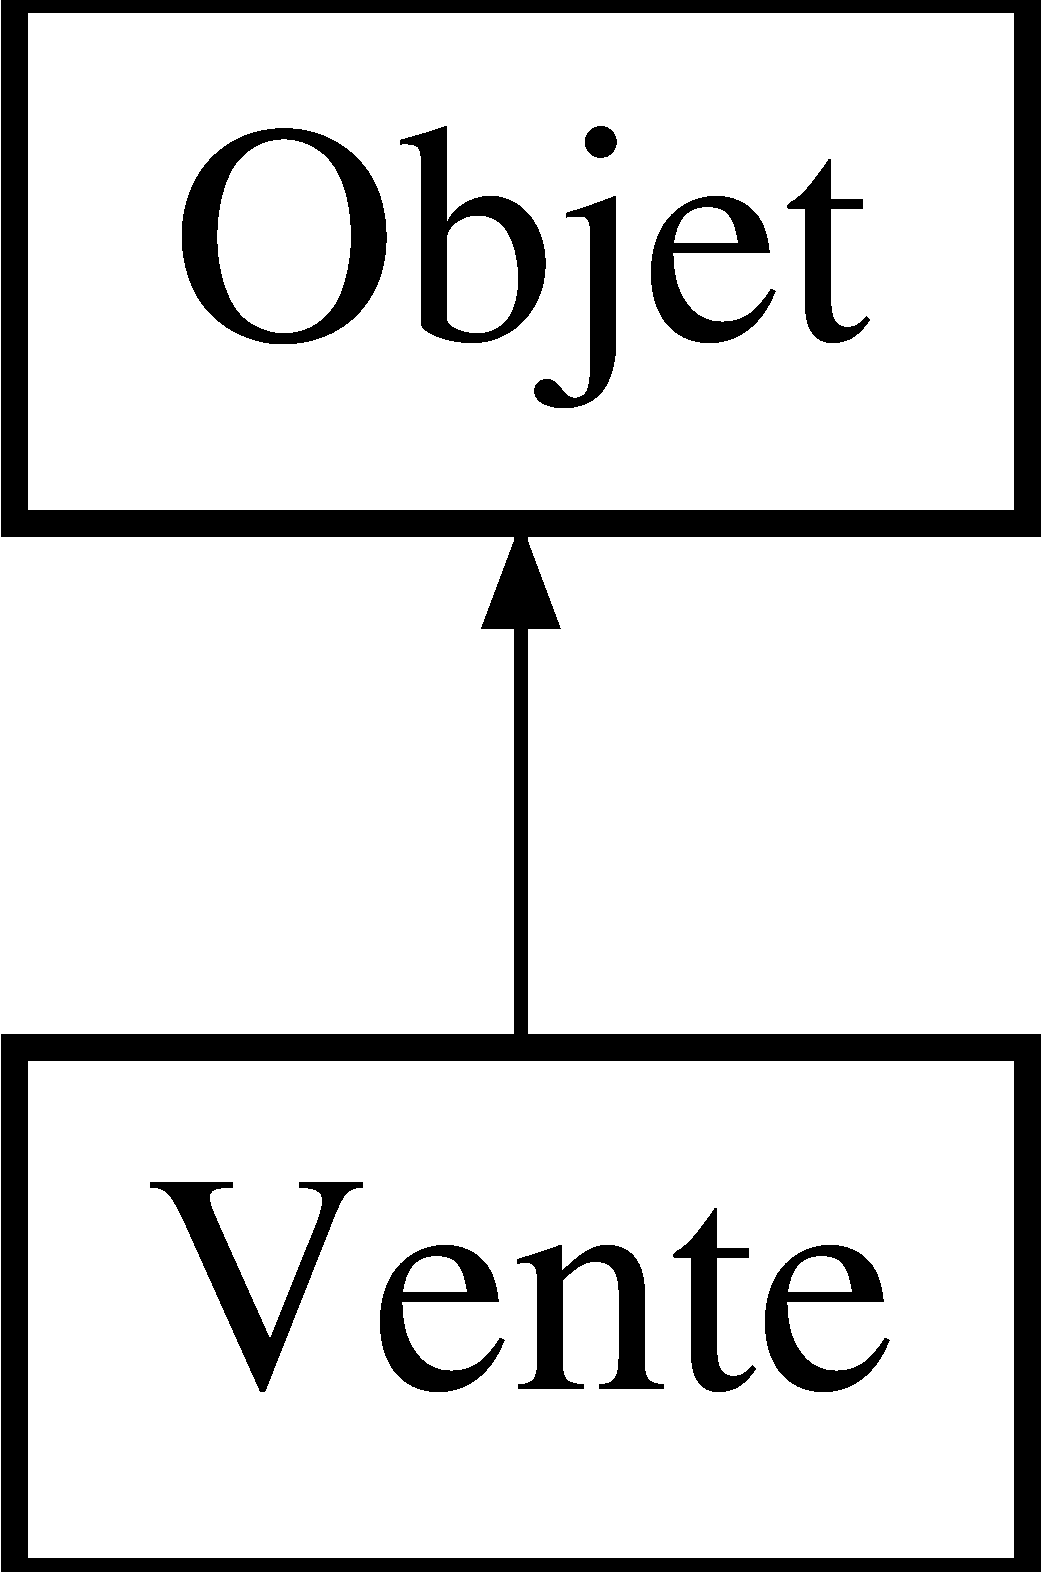
\includegraphics[height=2.000000cm]{class_objet}
\end{center}
\end{figure}


\subsection{Detailed Description}


Definition at line 7 of file objet.h.



The documentation for this class was generated from the following file:\begin{DoxyCompactItemize}
\item 
core/objet.h\end{DoxyCompactItemize}

\hypertarget{class_ordinateur}{
\section{Ordinateur Class Reference}
\label{class_ordinateur}\index{Ordinateur@{Ordinateur}}
}


\subsection{Detailed Description}


Definition at line 4 of file ordinateur.h.



The documentation for this class was generated from the following files:\begin{DoxyCompactItemize}
\item 
core/ordinateur.h\item 
core/ordinateur.cpp\end{DoxyCompactItemize}

\hypertarget{class_core_1_1_produit}{
\section{Référence de la classe Core::Produit}
\label{d3/d87/class_core_1_1_produit}\index{Core::Produit@{Core::Produit}}
}


Graphe d'héritage de Core::Produit:\nopagebreak
\begin{figure}[H]
\begin{center}
\leavevmode
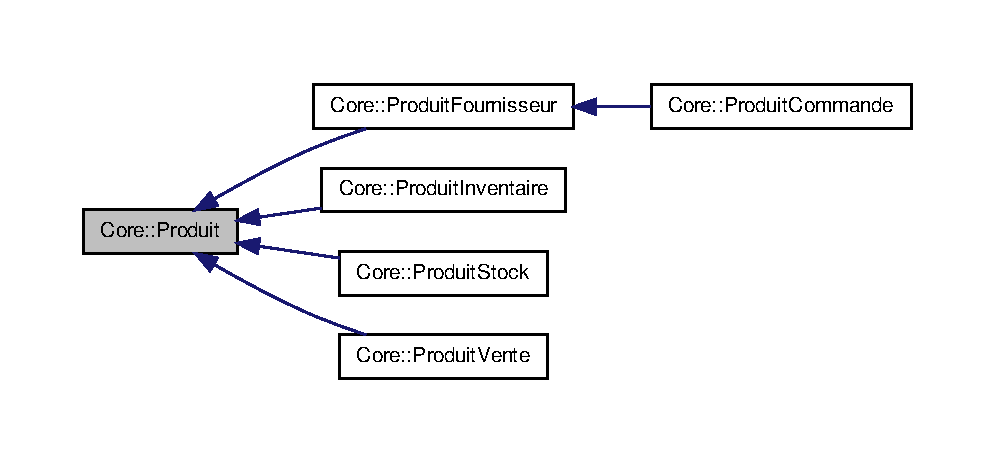
\includegraphics[width=400pt]{d3/dec/class_core_1_1_produit__inherit__graph}
\end{center}
\end{figure}
\subsection*{Fonctions membres publiques}
\begin{DoxyCompactItemize}
\item 
\hypertarget{class_core_1_1_produit_aa2985157600e8bcc14066d4a6c409b58}{
{\bfseries Produit} (QObject $\ast$parent=0)}
\label{d3/d87/class_core_1_1_produit_aa2985157600e8bcc14066d4a6c409b58}

\item 
\hypertarget{class_core_1_1_produit_af0d0d292e28cd8ca27716658085c8d06}{
{\bfseries Produit} (QString code, QObject $\ast$parent=0)}
\label{d3/d87/class_core_1_1_produit_af0d0d292e28cd8ca27716658085c8d06}

\item 
\hypertarget{class_core_1_1_produit_a08bff6e31a0d67b18c18871555ef4caa}{
{\bfseries Produit} (QString code, QString constructeur, QString nom, QString description, QObject $\ast$parent=0)}
\label{d3/d87/class_core_1_1_produit_a08bff6e31a0d67b18c18871555ef4caa}

\item 
\hypertarget{class_core_1_1_produit_a94212643b93f6299aff4b5a9b090f89c}{
QString {\bfseries getCode} () const }
\label{d3/d87/class_core_1_1_produit_a94212643b93f6299aff4b5a9b090f89c}

\item 
\hypertarget{class_core_1_1_produit_acf669ae426d5dc80b8600d23fffe64ed}{
QString {\bfseries getConstructeur} () const }
\label{d3/d87/class_core_1_1_produit_acf669ae426d5dc80b8600d23fffe64ed}

\item 
\hypertarget{class_core_1_1_produit_a2414900a8ab334bfc1cab191fe3abe12}{
QString {\bfseries getNom} () const }
\label{d3/d87/class_core_1_1_produit_a2414900a8ab334bfc1cab191fe3abe12}

\item 
\hypertarget{class_core_1_1_produit_a1afefe251b7e14c6d78f19f55fbdbc21}{
QString {\bfseries getDescription} () const }
\label{d3/d87/class_core_1_1_produit_a1afefe251b7e14c6d78f19f55fbdbc21}

\item 
\hypertarget{class_core_1_1_produit_a12f13870a2373d6a02517050cbd68a5b}{
void {\bfseries setCode} (QString code)}
\label{d3/d87/class_core_1_1_produit_a12f13870a2373d6a02517050cbd68a5b}

\item 
\hypertarget{class_core_1_1_produit_a690ce68de1f35f3f18363fabe8843a2a}{
void {\bfseries setConstructeur} (QString constructeur)}
\label{d3/d87/class_core_1_1_produit_a690ce68de1f35f3f18363fabe8843a2a}

\item 
\hypertarget{class_core_1_1_produit_ac6b8005023ed5b2fb55ecb323e45178c}{
void {\bfseries setNom} (QString nom)}
\label{d3/d87/class_core_1_1_produit_ac6b8005023ed5b2fb55ecb323e45178c}

\item 
\hypertarget{class_core_1_1_produit_ab52592d90eb5741c5ce0123bb7144942}{
void {\bfseries setDescription} (QString description)}
\label{d3/d87/class_core_1_1_produit_ab52592d90eb5741c5ce0123bb7144942}

\end{DoxyCompactItemize}
\subsection*{Propriétés}
\begin{DoxyCompactItemize}
\item 
\hypertarget{class_core_1_1_produit_a0aba1fa3c724c5869d1ba00f43895136}{
QString {\bfseries code}}
\label{d3/d87/class_core_1_1_produit_a0aba1fa3c724c5869d1ba00f43895136}

\item 
\hypertarget{class_core_1_1_produit_adb00517961528cadfb2ae7a2c91aebe3}{
QString {\bfseries constructeur}}
\label{d3/d87/class_core_1_1_produit_adb00517961528cadfb2ae7a2c91aebe3}

\item 
\hypertarget{class_core_1_1_produit_a99751d8e59c8bcca121479717c65cd07}{
QString {\bfseries nom}}
\label{d3/d87/class_core_1_1_produit_a99751d8e59c8bcca121479717c65cd07}

\item 
\hypertarget{class_core_1_1_produit_a2dd068f7aec5fe95cbbc2a8342a2b561}{
QString {\bfseries description}}
\label{d3/d87/class_core_1_1_produit_a2dd068f7aec5fe95cbbc2a8342a2b561}

\end{DoxyCompactItemize}


\subsection{Description détaillée}


Définition à la ligne 8 du fichier produit.h.



La documentation de cette classe a été générée à partir des fichiers suivants :\begin{DoxyCompactItemize}
\item 
core/produit.h\item 
core/produit.cpp\end{DoxyCompactItemize}

\hypertarget{class_core_1_1_produit_commande}{
\section{Référence de la classe Core::ProduitCommande}
\label{dc/d80/class_core_1_1_produit_commande}\index{Core::ProduitCommande@{Core::ProduitCommande}}
}


Graphe d'héritage de Core::ProduitCommande:\nopagebreak
\begin{figure}[H]
\begin{center}
\leavevmode
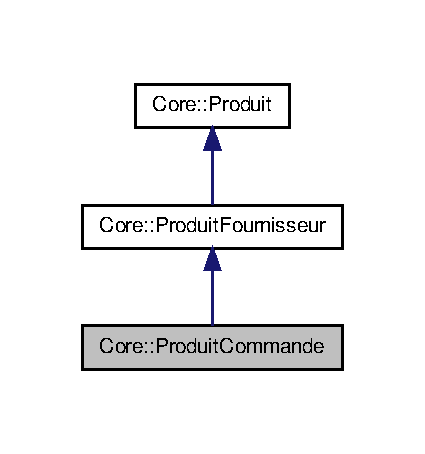
\includegraphics[width=204pt]{d3/d36/class_core_1_1_produit_commande__inherit__graph}
\end{center}
\end{figure}


Graphe de collaboration de Core::ProduitCommande:\nopagebreak
\begin{figure}[H]
\begin{center}
\leavevmode
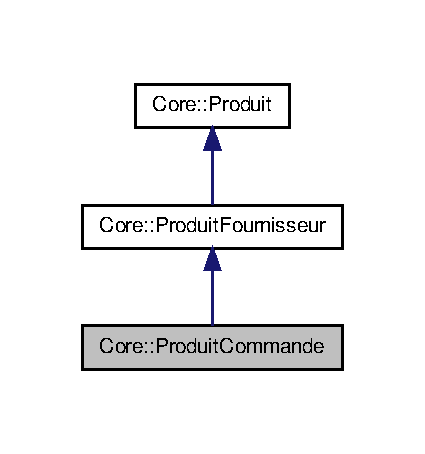
\includegraphics[width=204pt]{d4/d80/class_core_1_1_produit_commande__coll__graph}
\end{center}
\end{figure}
\subsection*{Fonctions membres publiques}
\begin{DoxyCompactItemize}
\item 
\hypertarget{class_core_1_1_produit_commande_a58fd9cc89c8cf3dcaddf9817952a2042}{
{\bfseries ProduitCommande} (QObject $\ast$parent=0)}
\label{dc/d80/class_core_1_1_produit_commande_a58fd9cc89c8cf3dcaddf9817952a2042}

\item 
\hypertarget{class_core_1_1_produit_commande_ab829e7b286f4712346170605dc4d5dae}{
int {\bfseries getQuantiteCommandee} () const }
\label{dc/d80/class_core_1_1_produit_commande_ab829e7b286f4712346170605dc4d5dae}

\item 
\hypertarget{class_core_1_1_produit_commande_afcd2572b808302456a86ffc7f53ea537}{
void {\bfseries setQuantiteCommandee} (int quantite)}
\label{dc/d80/class_core_1_1_produit_commande_afcd2572b808302456a86ffc7f53ea537}

\end{DoxyCompactItemize}
\subsection*{Propriétés}
\begin{DoxyCompactItemize}
\item 
\hypertarget{class_core_1_1_produit_commande_a241e17ad0ed66194629c1533d52673aa}{
int {\bfseries quantiteCommandee}}
\label{dc/d80/class_core_1_1_produit_commande_a241e17ad0ed66194629c1533d52673aa}

\end{DoxyCompactItemize}


\subsection{Description détaillée}


Définition à la ligne 8 du fichier produitcommande.h.



La documentation de cette classe a été générée à partir des fichiers suivants :\begin{DoxyCompactItemize}
\item 
core/produitcommande.h\item 
core/produitcommande.cpp\end{DoxyCompactItemize}

\hypertarget{class_core_1_1_produit_fournisseur}{
\section{Référence de la classe Core::ProduitFournisseur}
\label{d6/db3/class_core_1_1_produit_fournisseur}\index{Core::ProduitFournisseur@{Core::ProduitFournisseur}}
}


Graphe d'héritage de Core::ProduitFournisseur:\nopagebreak
\begin{figure}[H]
\begin{center}
\leavevmode
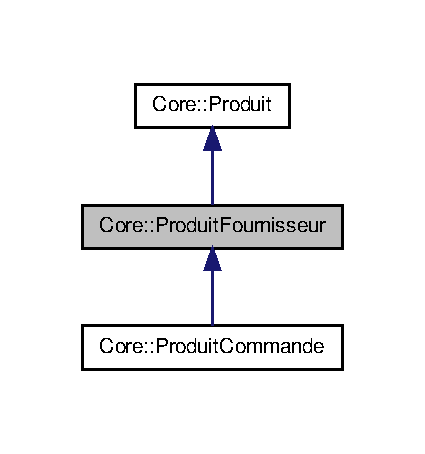
\includegraphics[width=204pt]{d9/d9d/class_core_1_1_produit_fournisseur__inherit__graph}
\end{center}
\end{figure}


Graphe de collaboration de Core::ProduitFournisseur:\nopagebreak
\begin{figure}[H]
\begin{center}
\leavevmode
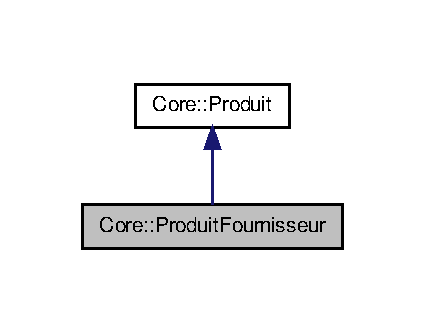
\includegraphics[width=204pt]{d4/d4a/class_core_1_1_produit_fournisseur__coll__graph}
\end{center}
\end{figure}
\subsection*{Fonctions membres publiques}
\begin{DoxyCompactItemize}
\item 
\hypertarget{class_core_1_1_produit_fournisseur_a98254017d4ef0541da1e4f4ea2701b71}{
{\bfseries ProduitFournisseur} (QObject $\ast$parent=0)}
\label{d6/db3/class_core_1_1_produit_fournisseur_a98254017d4ef0541da1e4f4ea2701b71}

\item 
\hypertarget{class_core_1_1_produit_fournisseur_a919a173e34c768151036aa2e48e62faf}{
{\bfseries ProduitFournisseur} (QString codeFournisseur, QObject $\ast$parent=0)}
\label{d6/db3/class_core_1_1_produit_fournisseur_a919a173e34c768151036aa2e48e62faf}

\item 
\hypertarget{class_core_1_1_produit_fournisseur_a100fb8ec0e64617842fdbaed117f8a42}{
QString {\bfseries getCodeFournisseur} () const }
\label{d6/db3/class_core_1_1_produit_fournisseur_a100fb8ec0e64617842fdbaed117f8a42}

\item 
\hypertarget{class_core_1_1_produit_fournisseur_a402bb9863ae2990179b6d135922d298d}{
double {\bfseries getPrixFournisseur} () const }
\label{d6/db3/class_core_1_1_produit_fournisseur_a402bb9863ae2990179b6d135922d298d}

\item 
\hypertarget{class_core_1_1_produit_fournisseur_a2a8047bfecd2ef16e08035ee49b63273}{
void {\bfseries setCodeFournisseur} (QString codeFournisseur)}
\label{d6/db3/class_core_1_1_produit_fournisseur_a2a8047bfecd2ef16e08035ee49b63273}

\item 
\hypertarget{class_core_1_1_produit_fournisseur_ab5b175a302d11050338b3f20624f913d}{
void {\bfseries setPrixFournisseur} (double prixFournisseur)}
\label{d6/db3/class_core_1_1_produit_fournisseur_ab5b175a302d11050338b3f20624f913d}

\end{DoxyCompactItemize}
\subsection*{Propriétés}
\begin{DoxyCompactItemize}
\item 
\hypertarget{class_core_1_1_produit_fournisseur_a7e89d7784e8627f76148c356505f705a}{
QString {\bfseries codeFournisseur}}
\label{d6/db3/class_core_1_1_produit_fournisseur_a7e89d7784e8627f76148c356505f705a}

\item 
\hypertarget{class_core_1_1_produit_fournisseur_a6938005393d9cc2b26475c1ce9f02f93}{
double {\bfseries prixFournisseur}}
\label{d6/db3/class_core_1_1_produit_fournisseur_a6938005393d9cc2b26475c1ce9f02f93}

\end{DoxyCompactItemize}


\subsection{Description détaillée}


Définition à la ligne 8 du fichier produitfournisseur.h.



La documentation de cette classe a été générée à partir des fichiers suivants :\begin{DoxyCompactItemize}
\item 
core/produitfournisseur.h\item 
core/produitfournisseur.cpp\end{DoxyCompactItemize}

\hypertarget{class_core_1_1_produit_inventaire}{
\section{Référence de la classe Core::ProduitInventaire}
\label{d4/d53/class_core_1_1_produit_inventaire}\index{Core::ProduitInventaire@{Core::ProduitInventaire}}
}


Graphe d'héritage de Core::ProduitInventaire:\nopagebreak
\begin{figure}[H]
\begin{center}
\leavevmode
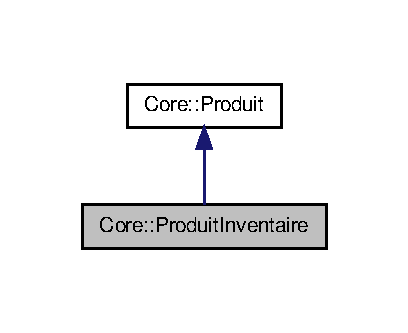
\includegraphics[width=196pt]{d8/d1c/class_core_1_1_produit_inventaire__inherit__graph}
\end{center}
\end{figure}


Graphe de collaboration de Core::ProduitInventaire:\nopagebreak
\begin{figure}[H]
\begin{center}
\leavevmode
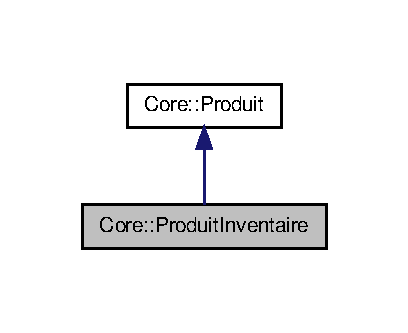
\includegraphics[width=196pt]{da/dd7/class_core_1_1_produit_inventaire__coll__graph}
\end{center}
\end{figure}
\subsection*{Types publics}
\begin{DoxyCompactItemize}
\item 
enum {\bfseries Etat} \{ {\bfseries BonEtat}, 
{\bfseries Deteriore}, 
{\bfseries Vole}
 \}
\end{DoxyCompactItemize}
\subsection*{Fonctions membres publiques}
\begin{DoxyCompactItemize}
\item 
\hypertarget{class_core_1_1_produit_inventaire_a9e523fdd7b5989520a88066561017121}{
{\bfseries ProduitInventaire} (QObject $\ast$parent=0)}
\label{d4/d53/class_core_1_1_produit_inventaire_a9e523fdd7b5989520a88066561017121}

\item 
\hypertarget{class_core_1_1_produit_inventaire_a10e08d895e2513a59fea74e580aac7e8}{
int {\bfseries getQuantite} () const }
\label{d4/d53/class_core_1_1_produit_inventaire_a10e08d895e2513a59fea74e580aac7e8}

\item 
\hypertarget{class_core_1_1_produit_inventaire_ad5dd92f4476fad4757cb10462f4eefb1}{
int {\bfseries getEtat} () const }
\label{d4/d53/class_core_1_1_produit_inventaire_ad5dd92f4476fad4757cb10462f4eefb1}

\item 
\hypertarget{class_core_1_1_produit_inventaire_a59d68c5950101aa30a9ce8dc7a4b0e45}{
void {\bfseries setQuantite} (int quantite)}
\label{d4/d53/class_core_1_1_produit_inventaire_a59d68c5950101aa30a9ce8dc7a4b0e45}

\item 
\hypertarget{class_core_1_1_produit_inventaire_aff84b8ce540258afbbfb958fd54ed316}{
void {\bfseries setEtat} (int etat)}
\label{d4/d53/class_core_1_1_produit_inventaire_aff84b8ce540258afbbfb958fd54ed316}

\end{DoxyCompactItemize}
\subsection*{Propriétés}
\begin{DoxyCompactItemize}
\item 
\hypertarget{class_core_1_1_produit_inventaire_a7059db71032dbbeb3391fd6fdd6d9ea7}{
int {\bfseries quantite}}
\label{d4/d53/class_core_1_1_produit_inventaire_a7059db71032dbbeb3391fd6fdd6d9ea7}

\item 
\hypertarget{class_core_1_1_produit_inventaire_af550b34aacf39149fc19257bcb990b27}{
int {\bfseries etat}}
\label{d4/d53/class_core_1_1_produit_inventaire_af550b34aacf39149fc19257bcb990b27}

\end{DoxyCompactItemize}


\subsection{Description détaillée}


Définition à la ligne 8 du fichier produitinventaire.h.



La documentation de cette classe a été générée à partir des fichiers suivants :\begin{DoxyCompactItemize}
\item 
core/produitinventaire.h\item 
core/produitinventaire.cpp\end{DoxyCompactItemize}

\hypertarget{class_core_1_1_produit_stock}{
\section{Référence de la classe Core::ProduitStock}
\label{d6/d92/class_core_1_1_produit_stock}\index{Core::ProduitStock@{Core::ProduitStock}}
}


Graphe d'héritage de Core::ProduitStock:\nopagebreak
\begin{figure}[H]
\begin{center}
\leavevmode
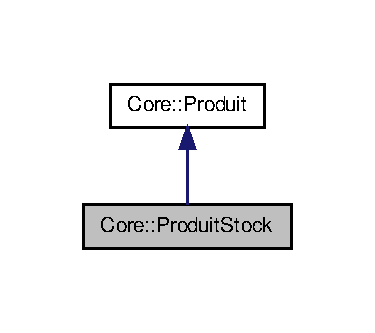
\includegraphics[width=180pt]{d2/dee/class_core_1_1_produit_stock__inherit__graph}
\end{center}
\end{figure}


Graphe de collaboration de Core::ProduitStock:\nopagebreak
\begin{figure}[H]
\begin{center}
\leavevmode
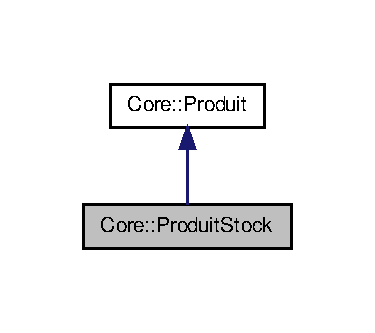
\includegraphics[width=180pt]{d7/d71/class_core_1_1_produit_stock__coll__graph}
\end{center}
\end{figure}
\subsection*{Fonctions membres publiques}
\begin{DoxyCompactItemize}
\item 
\hypertarget{class_core_1_1_produit_stock_a08ab8dd30ad1be969c9188e2195346fc}{
{\bfseries ProduitStock} (QObject $\ast$parent=0)}
\label{d6/d92/class_core_1_1_produit_stock_a08ab8dd30ad1be969c9188e2195346fc}

\item 
\hypertarget{class_core_1_1_produit_stock_a5f04709d621122123c9117d825a94283}{
{\bfseries ProduitStock} (QString code)}
\label{d6/d92/class_core_1_1_produit_stock_a5f04709d621122123c9117d825a94283}

\item 
\hypertarget{class_core_1_1_produit_stock_a5f4b935a17a0b0435b8c34ae5760abfd}{
int {\bfseries getQuantite} () const }
\label{d6/d92/class_core_1_1_produit_stock_a5f4b935a17a0b0435b8c34ae5760abfd}

\item 
\hypertarget{class_core_1_1_produit_stock_a16263756453a8edffa89cb67eb80b575}{
double {\bfseries getPrixUnitaire} () const }
\label{d6/d92/class_core_1_1_produit_stock_a16263756453a8edffa89cb67eb80b575}

\item 
\hypertarget{class_core_1_1_produit_stock_aa7d1dbc31ea1bf622493cf98f7f06592}{
void {\bfseries setQuantite} (int quantite)}
\label{d6/d92/class_core_1_1_produit_stock_aa7d1dbc31ea1bf622493cf98f7f06592}

\item 
\hypertarget{class_core_1_1_produit_stock_a4110dd03fd5622936a6ac1c281aa157a}{
void {\bfseries setPrixUnitaire} (double prixUnitaire)}
\label{d6/d92/class_core_1_1_produit_stock_a4110dd03fd5622936a6ac1c281aa157a}

\end{DoxyCompactItemize}
\subsection*{Propriétés}
\begin{DoxyCompactItemize}
\item 
\hypertarget{class_core_1_1_produit_stock_a13e71c5d6ab069975dc3452a4359d08e}{
int {\bfseries quantite}}
\label{d6/d92/class_core_1_1_produit_stock_a13e71c5d6ab069975dc3452a4359d08e}

\item 
\hypertarget{class_core_1_1_produit_stock_aea5b4f63bd0bdb3f4add70bad70fc889}{
double {\bfseries prixUnitaire}}
\label{d6/d92/class_core_1_1_produit_stock_aea5b4f63bd0bdb3f4add70bad70fc889}

\end{DoxyCompactItemize}


\subsection{Description détaillée}


Définition à la ligne 8 du fichier produitstock.h.



La documentation de cette classe a été générée à partir des fichiers suivants :\begin{DoxyCompactItemize}
\item 
core/produitstock.h\item 
core/produitstock.cpp\end{DoxyCompactItemize}

\hypertarget{class_core_1_1_produit_vente}{
\section{Référence de la classe Core::ProduitVente}
\label{d3/d4f/class_core_1_1_produit_vente}\index{Core::ProduitVente@{Core::ProduitVente}}
}


Graphe d'héritage de Core::ProduitVente:\nopagebreak
\begin{figure}[H]
\begin{center}
\leavevmode
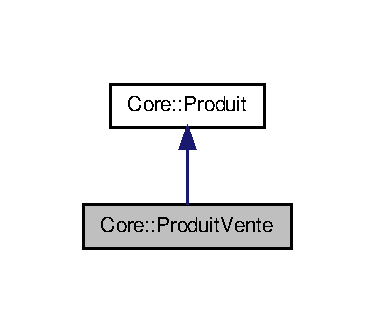
\includegraphics[width=180pt]{d1/d35/class_core_1_1_produit_vente__inherit__graph}
\end{center}
\end{figure}


Graphe de collaboration de Core::ProduitVente:\nopagebreak
\begin{figure}[H]
\begin{center}
\leavevmode
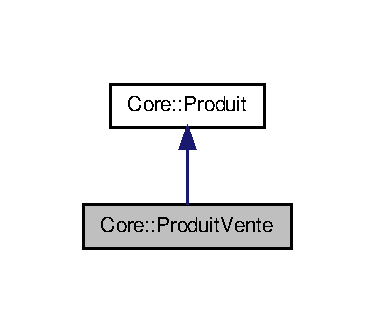
\includegraphics[width=180pt]{da/d70/class_core_1_1_produit_vente__coll__graph}
\end{center}
\end{figure}
\subsection*{Fonctions membres publiques}
\begin{DoxyCompactItemize}
\item 
\hypertarget{class_core_1_1_produit_vente_acc72c533d8369d796efada34338ca196}{
{\bfseries ProduitVente} (QObject $\ast$parent=0)}
\label{d3/d4f/class_core_1_1_produit_vente_acc72c533d8369d796efada34338ca196}

\item 
\hypertarget{class_core_1_1_produit_vente_af9a077f070b97bdc21a58c836b74e616}{
{\bfseries ProduitVente} (QString code, QObject $\ast$parent=0)}
\label{d3/d4f/class_core_1_1_produit_vente_af9a077f070b97bdc21a58c836b74e616}

\item 
\hypertarget{class_core_1_1_produit_vente_a3da7b36ef38ff110d4a2ce8d42af723d}{
double {\bfseries getPrixUnitaire} () const }
\label{d3/d4f/class_core_1_1_produit_vente_a3da7b36ef38ff110d4a2ce8d42af723d}

\item 
\hypertarget{class_core_1_1_produit_vente_a349a1d192d301398d84ba5bf875f7a03}{
int {\bfseries getQuantiteVendue} () const }
\label{d3/d4f/class_core_1_1_produit_vente_a349a1d192d301398d84ba5bf875f7a03}

\item 
\hypertarget{class_core_1_1_produit_vente_a41a15298072493461f18d6161286100e}{
void {\bfseries setPrixUnitaire} (double prixUnitaire)}
\label{d3/d4f/class_core_1_1_produit_vente_a41a15298072493461f18d6161286100e}

\item 
\hypertarget{class_core_1_1_produit_vente_a451fa2e0bba35498cb525e3c905ce476}{
void {\bfseries setQuantiteVendue} (int quantiteVendue)}
\label{d3/d4f/class_core_1_1_produit_vente_a451fa2e0bba35498cb525e3c905ce476}

\end{DoxyCompactItemize}
\subsection*{Propriétés}
\begin{DoxyCompactItemize}
\item 
\hypertarget{class_core_1_1_produit_vente_ac1bf22361ff20e2c42ddff825d8941b3}{
int {\bfseries quantiteVendue}}
\label{d3/d4f/class_core_1_1_produit_vente_ac1bf22361ff20e2c42ddff825d8941b3}

\item 
\hypertarget{class_core_1_1_produit_vente_aa979cd9cc655cfbd93648ab136ffe68e}{
double {\bfseries prixUnitaire}}
\label{d3/d4f/class_core_1_1_produit_vente_aa979cd9cc655cfbd93648ab136ffe68e}

\end{DoxyCompactItemize}


\subsection{Description détaillée}


Définition à la ligne 8 du fichier produitvente.h.



La documentation de cette classe a été générée à partir des fichiers suivants :\begin{DoxyCompactItemize}
\item 
core/produitvente.h\item 
core/produitvente.cpp\end{DoxyCompactItemize}

\hypertarget{class_core_1_1_r_produit_catalogue}{
\section{Référence de la classe Core::RProduitCatalogue}
\label{dd/da1/class_core_1_1_r_produit_catalogue}\index{Core::RProduitCatalogue@{Core::RProduitCatalogue}}
}


Graphe de collaboration de Core::RProduitCatalogue:\nopagebreak
\begin{figure}[H]
\begin{center}
\leavevmode
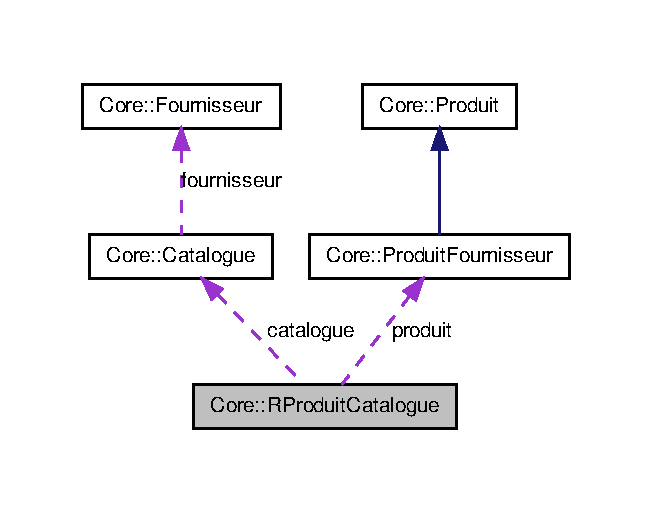
\includegraphics[width=313pt]{d8/da1/class_core_1_1_r_produit_catalogue__coll__graph}
\end{center}
\end{figure}
\subsection*{Fonctions membres publiques}
\begin{DoxyCompactItemize}
\item 
\hypertarget{class_core_1_1_r_produit_catalogue_a3d0a600af8d4f47ef97c0bf20ee8664f}{
{\bfseries RProduitCatalogue} (QObject $\ast$parent=0)}
\label{dd/da1/class_core_1_1_r_produit_catalogue_a3d0a600af8d4f47ef97c0bf20ee8664f}

\item 
\hypertarget{class_core_1_1_r_produit_catalogue_a6bab4ba1c2a9f71b5c207d5404e79818}{
\hyperlink{class_core_1_1_catalogue}{Catalogue} $\ast$ {\bfseries getCatalogue} () const }
\label{dd/da1/class_core_1_1_r_produit_catalogue_a6bab4ba1c2a9f71b5c207d5404e79818}

\item 
\hypertarget{class_core_1_1_r_produit_catalogue_abaecabf9417832733b9c246ac7ff3462}{
\hyperlink{class_core_1_1_produit_fournisseur}{ProduitFournisseur} $\ast$ {\bfseries getProduit} () const }
\label{dd/da1/class_core_1_1_r_produit_catalogue_abaecabf9417832733b9c246ac7ff3462}

\item 
\hypertarget{class_core_1_1_r_produit_catalogue_a2f81ff93493d17457a5f311087345957}{
void {\bfseries setCatalogue} (\hyperlink{class_core_1_1_catalogue}{Catalogue} $\ast$catalogue)}
\label{dd/da1/class_core_1_1_r_produit_catalogue_a2f81ff93493d17457a5f311087345957}

\item 
\hypertarget{class_core_1_1_r_produit_catalogue_a6754409e8b03a601476b9d41985a8c12}{
void {\bfseries setProduit} (\hyperlink{class_core_1_1_produit_fournisseur}{ProduitFournisseur} $\ast$produit)}
\label{dd/da1/class_core_1_1_r_produit_catalogue_a6754409e8b03a601476b9d41985a8c12}

\item 
\hypertarget{class_core_1_1_r_produit_catalogue_a529594a38233941c5e8f9d9a28a557b1}{
bool {\bfseries save} ()}
\label{dd/da1/class_core_1_1_r_produit_catalogue_a529594a38233941c5e8f9d9a28a557b1}

\end{DoxyCompactItemize}
\subsection*{Propriétés}
\begin{DoxyCompactItemize}
\item 
\hypertarget{class_core_1_1_r_produit_catalogue_a85a088d3320fe97e316088fb7aaf3089}{
QString {\bfseries id}}
\label{dd/da1/class_core_1_1_r_produit_catalogue_a85a088d3320fe97e316088fb7aaf3089}

\item 
\hypertarget{class_core_1_1_r_produit_catalogue_a93913cd4c0bb6ee0c14d5edea3e72262}{
\hyperlink{class_core_1_1_catalogue}{Catalogue} {\bfseries catalogue}}
\label{dd/da1/class_core_1_1_r_produit_catalogue_a93913cd4c0bb6ee0c14d5edea3e72262}

\item 
\hypertarget{class_core_1_1_r_produit_catalogue_a42bd407f297a089a0bfc2767923cb4ae}{
\hyperlink{class_core_1_1_produit_fournisseur}{ProduitFournisseur} {\bfseries produit}}
\label{dd/da1/class_core_1_1_r_produit_catalogue_a42bd407f297a089a0bfc2767923cb4ae}

\end{DoxyCompactItemize}


\subsection{Description détaillée}


Définition à la ligne 9 du fichier rproduitcatalogue.h.



La documentation de cette classe a été générée à partir des fichiers suivants :\begin{DoxyCompactItemize}
\item 
core/rproduitcatalogue.h\item 
core/rproduitcatalogue.cpp\end{DoxyCompactItemize}

\hypertarget{class_core_1_1_r_produit_commande}{
\section{Référence de la classe Core::RProduitCommande}
\label{d3/dad/class_core_1_1_r_produit_commande}\index{Core::RProduitCommande@{Core::RProduitCommande}}
}


Graphe de collaboration de Core::RProduitCommande:\nopagebreak
\begin{figure}[H]
\begin{center}
\leavevmode
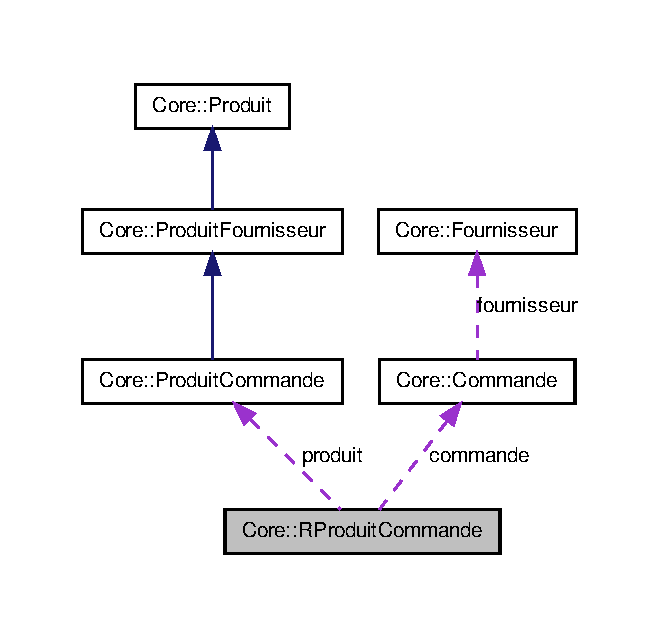
\includegraphics[width=318pt]{d3/dbc/class_core_1_1_r_produit_commande__coll__graph}
\end{center}
\end{figure}
\subsection*{Fonctions membres publiques}
\begin{DoxyCompactItemize}
\item 
\hypertarget{class_core_1_1_r_produit_commande_a2e9cd2c0387b6afffa295ae84b2e8c26}{
{\bfseries RProduitCommande} (QObject $\ast$parent=0)}
\label{d3/dad/class_core_1_1_r_produit_commande_a2e9cd2c0387b6afffa295ae84b2e8c26}

\item 
\hypertarget{class_core_1_1_r_produit_commande_ae158ca7581b66a19754333f503a84186}{
\hyperlink{class_core_1_1_commande}{Commande} $\ast$ {\bfseries getCommande} () const }
\label{d3/dad/class_core_1_1_r_produit_commande_ae158ca7581b66a19754333f503a84186}

\item 
\hypertarget{class_core_1_1_r_produit_commande_a16358dc859df69c57ee839baf5a5e649}{
\hyperlink{class_core_1_1_produit_commande}{ProduitCommande} $\ast$ {\bfseries getProduit} () const }
\label{d3/dad/class_core_1_1_r_produit_commande_a16358dc859df69c57ee839baf5a5e649}

\item 
\hypertarget{class_core_1_1_r_produit_commande_a0dff00840852b994f29929bf3731812e}{
void {\bfseries setCommande} (\hyperlink{class_core_1_1_commande}{Commande} $\ast$commande)}
\label{d3/dad/class_core_1_1_r_produit_commande_a0dff00840852b994f29929bf3731812e}

\item 
\hypertarget{class_core_1_1_r_produit_commande_af2ee8a58992da03e17d2a6864d620519}{
void {\bfseries setProduit} (\hyperlink{class_core_1_1_produit_commande}{ProduitCommande} $\ast$produit)}
\label{d3/dad/class_core_1_1_r_produit_commande_af2ee8a58992da03e17d2a6864d620519}

\item 
\hypertarget{class_core_1_1_r_produit_commande_a5ea11f38293ac9d03019368f808c19c3}{
bool {\bfseries save} ()}
\label{d3/dad/class_core_1_1_r_produit_commande_a5ea11f38293ac9d03019368f808c19c3}

\end{DoxyCompactItemize}
\subsection*{Propriétés}
\begin{DoxyCompactItemize}
\item 
\hypertarget{class_core_1_1_r_produit_commande_a6b94e74d9e458754516f549dcbfbcf8a}{
QString {\bfseries id}}
\label{d3/dad/class_core_1_1_r_produit_commande_a6b94e74d9e458754516f549dcbfbcf8a}

\item 
\hypertarget{class_core_1_1_r_produit_commande_afacfd78cc1baa69c78b150485e5bb92a}{
\hyperlink{class_core_1_1_commande}{Commande} {\bfseries commande}}
\label{d3/dad/class_core_1_1_r_produit_commande_afacfd78cc1baa69c78b150485e5bb92a}

\item 
\hypertarget{class_core_1_1_r_produit_commande_a2480c7e336c78bbc46bc9bb2813abcff}{
\hyperlink{class_core_1_1_produit_commande}{ProduitCommande} {\bfseries produit}}
\label{d3/dad/class_core_1_1_r_produit_commande_a2480c7e336c78bbc46bc9bb2813abcff}

\end{DoxyCompactItemize}


\subsection{Description détaillée}


Définition à la ligne 9 du fichier rproduitcommande.h.



La documentation de cette classe a été générée à partir des fichiers suivants :\begin{DoxyCompactItemize}
\item 
core/rproduitcommande.h\item 
core/rproduitcommande.cpp\end{DoxyCompactItemize}

\hypertarget{class_core_1_1_r_produit_inventaire}{
\section{Référence de la classe Core::RProduitInventaire}
\label{d0/de7/class_core_1_1_r_produit_inventaire}\index{Core::RProduitInventaire@{Core::RProduitInventaire}}
}


Graphe de collaboration de Core::RProduitInventaire:\nopagebreak
\begin{figure}[H]
\begin{center}
\leavevmode
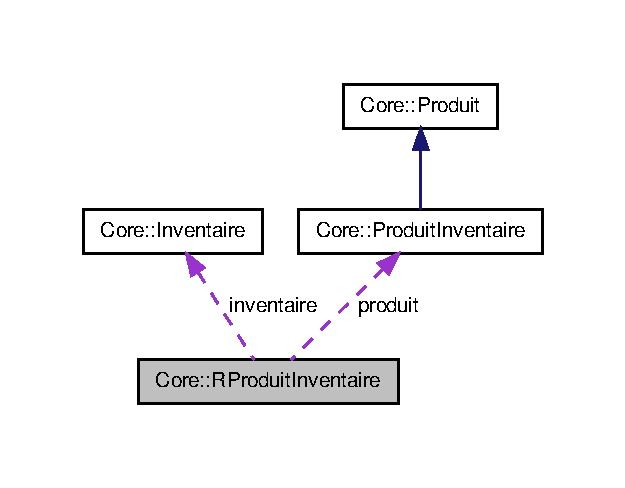
\includegraphics[width=300pt]{d3/d23/class_core_1_1_r_produit_inventaire__coll__graph}
\end{center}
\end{figure}
\subsection*{Fonctions membres publiques}
\begin{DoxyCompactItemize}
\item 
\hypertarget{class_core_1_1_r_produit_inventaire_a1569e6767ffac46a4b48d83b4d4c1a54}{
{\bfseries RProduitInventaire} (QObject $\ast$parent=0)}
\label{d0/de7/class_core_1_1_r_produit_inventaire_a1569e6767ffac46a4b48d83b4d4c1a54}

\item 
\hypertarget{class_core_1_1_r_produit_inventaire_a984a57da425c7cbeac7193a3be063038}{
\hyperlink{class_core_1_1_inventaire}{Inventaire} $\ast$ {\bfseries getInventaire} () const }
\label{d0/de7/class_core_1_1_r_produit_inventaire_a984a57da425c7cbeac7193a3be063038}

\item 
\hypertarget{class_core_1_1_r_produit_inventaire_ad8075fd3f61308efb03f23b84875c753}{
\hyperlink{class_core_1_1_produit_inventaire}{ProduitInventaire} $\ast$ {\bfseries getProduit} () const }
\label{d0/de7/class_core_1_1_r_produit_inventaire_ad8075fd3f61308efb03f23b84875c753}

\item 
\hypertarget{class_core_1_1_r_produit_inventaire_a1e2ef392d267fa50537f36b3396c04f6}{
void {\bfseries setInventaire} (\hyperlink{class_core_1_1_inventaire}{Inventaire} $\ast$inventaire)}
\label{d0/de7/class_core_1_1_r_produit_inventaire_a1e2ef392d267fa50537f36b3396c04f6}

\item 
\hypertarget{class_core_1_1_r_produit_inventaire_aaab3cc17bff56907bce7fb5752200971}{
void {\bfseries setProduit} (\hyperlink{class_core_1_1_produit_inventaire}{ProduitInventaire} $\ast$produit)}
\label{d0/de7/class_core_1_1_r_produit_inventaire_aaab3cc17bff56907bce7fb5752200971}

\item 
\hypertarget{class_core_1_1_r_produit_inventaire_a3a71392642e7bf29a2f09e989039a0f6}{
bool {\bfseries save} ()}
\label{d0/de7/class_core_1_1_r_produit_inventaire_a3a71392642e7bf29a2f09e989039a0f6}

\end{DoxyCompactItemize}
\subsection*{Propriétés}
\begin{DoxyCompactItemize}
\item 
\hypertarget{class_core_1_1_r_produit_inventaire_a3876ef2353d749ee6532b071d445f90a}{
QString {\bfseries id}}
\label{d0/de7/class_core_1_1_r_produit_inventaire_a3876ef2353d749ee6532b071d445f90a}

\item 
\hypertarget{class_core_1_1_r_produit_inventaire_a3606e4f9075928c283a29c50a53c4e29}{
\hyperlink{class_core_1_1_inventaire}{Inventaire} {\bfseries inventaire}}
\label{d0/de7/class_core_1_1_r_produit_inventaire_a3606e4f9075928c283a29c50a53c4e29}

\item 
\hypertarget{class_core_1_1_r_produit_inventaire_a557a668687200199217116c38142039d}{
\hyperlink{class_core_1_1_produit_inventaire}{ProduitInventaire} {\bfseries produit}}
\label{d0/de7/class_core_1_1_r_produit_inventaire_a557a668687200199217116c38142039d}

\end{DoxyCompactItemize}


\subsection{Description détaillée}


Définition à la ligne 9 du fichier rproduitinventaire.h.



La documentation de cette classe a été générée à partir des fichiers suivants :\begin{DoxyCompactItemize}
\item 
core/rproduitinventaire.h\item 
core/rproduitinventaire.cpp\end{DoxyCompactItemize}

\hypertarget{class_core_1_1_r_produit_stock}{
\section{Référence de la classe Core::RProduitStock}
\label{d1/da9/class_core_1_1_r_produit_stock}\index{Core::RProduitStock@{Core::RProduitStock}}
}


Graphe de collaboration de Core::RProduitStock:\nopagebreak
\begin{figure}[H]
\begin{center}
\leavevmode
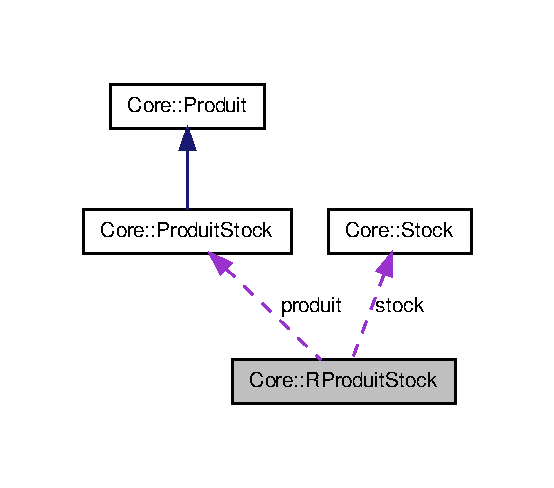
\includegraphics[width=266pt]{d4/d21/class_core_1_1_r_produit_stock__coll__graph}
\end{center}
\end{figure}
\subsection*{Fonctions membres publiques}
\begin{DoxyCompactItemize}
\item 
\hypertarget{class_core_1_1_r_produit_stock_ac660f4e216aec2988859d758787aa721}{
{\bfseries RProduitStock} (QObject $\ast$parent=0)}
\label{d1/da9/class_core_1_1_r_produit_stock_ac660f4e216aec2988859d758787aa721}

\item 
\hypertarget{class_core_1_1_r_produit_stock_aff8d6d51552239ba9e58fcf4c64f2453}{
\hyperlink{class_core_1_1_stock}{Stock} $\ast$ {\bfseries getStock} () const }
\label{d1/da9/class_core_1_1_r_produit_stock_aff8d6d51552239ba9e58fcf4c64f2453}

\item 
\hypertarget{class_core_1_1_r_produit_stock_ad7a6991f9312de5682f55999d146e5cb}{
\hyperlink{class_core_1_1_produit_stock}{ProduitStock} $\ast$ {\bfseries getProduit} () const }
\label{d1/da9/class_core_1_1_r_produit_stock_ad7a6991f9312de5682f55999d146e5cb}

\item 
\hypertarget{class_core_1_1_r_produit_stock_ae30f5b0ae401b2982efc10264d26ac57}{
void {\bfseries setStock} (\hyperlink{class_core_1_1_stock}{Stock} $\ast$stock)}
\label{d1/da9/class_core_1_1_r_produit_stock_ae30f5b0ae401b2982efc10264d26ac57}

\item 
\hypertarget{class_core_1_1_r_produit_stock_ac5dfc4e4d36e9181c5a71dfff31d7c5d}{
void {\bfseries setProduit} (\hyperlink{class_core_1_1_produit_stock}{ProduitStock} $\ast$produit)}
\label{d1/da9/class_core_1_1_r_produit_stock_ac5dfc4e4d36e9181c5a71dfff31d7c5d}

\item 
\hypertarget{class_core_1_1_r_produit_stock_af51256847809128d3fcb0a5853d47966}{
bool {\bfseries save} ()}
\label{d1/da9/class_core_1_1_r_produit_stock_af51256847809128d3fcb0a5853d47966}

\end{DoxyCompactItemize}
\subsection*{Propriétés}
\begin{DoxyCompactItemize}
\item 
\hypertarget{class_core_1_1_r_produit_stock_a48b9c66f04252b177f8c5f065c5eb47b}{
QString {\bfseries id}}
\label{d1/da9/class_core_1_1_r_produit_stock_a48b9c66f04252b177f8c5f065c5eb47b}

\item 
\hypertarget{class_core_1_1_r_produit_stock_ab988f08c75b5ad3d6eb61c46c55f9e42}{
\hyperlink{class_core_1_1_stock}{Stock} {\bfseries stock}}
\label{d1/da9/class_core_1_1_r_produit_stock_ab988f08c75b5ad3d6eb61c46c55f9e42}

\item 
\hypertarget{class_core_1_1_r_produit_stock_a2e242532e943af64cd35f83e53eb8d94}{
\hyperlink{class_core_1_1_produit_stock}{ProduitStock} {\bfseries produit}}
\label{d1/da9/class_core_1_1_r_produit_stock_a2e242532e943af64cd35f83e53eb8d94}

\end{DoxyCompactItemize}


\subsection{Description détaillée}


Définition à la ligne 9 du fichier rproduitstock.h.



La documentation de cette classe a été générée à partir des fichiers suivants :\begin{DoxyCompactItemize}
\item 
core/rproduitstock.h\item 
core/rproduitstock.cpp\end{DoxyCompactItemize}

\hypertarget{class_core_1_1_stock}{
\section{Référence de la classe Core::Stock}
\label{d6/d24/class_core_1_1_stock}\index{Core::Stock@{Core::Stock}}
}
\subsection*{Fonctions membres publiques}
\begin{DoxyCompactItemize}
\item 
\hypertarget{class_core_1_1_stock_a7e43366f550c98967452b84b38f5a13e}{
{\bfseries Stock} (QObject $\ast$parent=0)}
\label{d6/d24/class_core_1_1_stock_a7e43366f550c98967452b84b38f5a13e}

\item 
\hypertarget{class_core_1_1_stock_a3649191630c111a52193c1fd9d7b49a6}{
{\bfseries Stock} (QString code, QObject $\ast$parent=0)}
\label{d6/d24/class_core_1_1_stock_a3649191630c111a52193c1fd9d7b49a6}

\item 
\hypertarget{class_core_1_1_stock_ad2ce1820273694d0489070011523c8f2}{
QString {\bfseries getCode} () const }
\label{d6/d24/class_core_1_1_stock_ad2ce1820273694d0489070011523c8f2}

\item 
\hypertarget{class_core_1_1_stock_a58368d4a798eddf98bcc9f569a98bb38}{
QString {\bfseries getNom} () const }
\label{d6/d24/class_core_1_1_stock_a58368d4a798eddf98bcc9f569a98bb38}

\item 
\hypertarget{class_core_1_1_stock_a4252cfe8c43d71b0445100f4fe63f71d}{
QDate {\bfseries getDateCreation} () const }
\label{d6/d24/class_core_1_1_stock_a4252cfe8c43d71b0445100f4fe63f71d}

\item 
\hypertarget{class_core_1_1_stock_a4b66ba01a2da6ec009a28c56f414a5f2}{
void {\bfseries setCode} (QString code)}
\label{d6/d24/class_core_1_1_stock_a4b66ba01a2da6ec009a28c56f414a5f2}

\item 
\hypertarget{class_core_1_1_stock_a60200b3fe0f0e056fd1a145b78c8b221}{
void {\bfseries setNom} (QString nom)}
\label{d6/d24/class_core_1_1_stock_a60200b3fe0f0e056fd1a145b78c8b221}

\item 
\hypertarget{class_core_1_1_stock_a3621ce64a24b1abe3867e6772f8eae7f}{
void {\bfseries setDateCreation} (QDate dateCreation)}
\label{d6/d24/class_core_1_1_stock_a3621ce64a24b1abe3867e6772f8eae7f}

\end{DoxyCompactItemize}
\subsection*{Propriétés}
\begin{DoxyCompactItemize}
\item 
\hypertarget{class_core_1_1_stock_a0b685816b48d59f6aa5aa149fec7d70e}{
QString {\bfseries code}}
\label{d6/d24/class_core_1_1_stock_a0b685816b48d59f6aa5aa149fec7d70e}

\item 
\hypertarget{class_core_1_1_stock_a1e1402caa5271ecee32a2e86f26f8223}{
QString {\bfseries nom}}
\label{d6/d24/class_core_1_1_stock_a1e1402caa5271ecee32a2e86f26f8223}

\item 
\hypertarget{class_core_1_1_stock_a8ad2b7a5946a36b7f6afc3e3fd7a6abb}{
QDate {\bfseries dateCreation}}
\label{d6/d24/class_core_1_1_stock_a8ad2b7a5946a36b7f6afc3e3fd7a6abb}

\end{DoxyCompactItemize}


\subsection{Description détaillée}


Définition à la ligne 8 du fichier stock.h.



La documentation de cette classe a été générée à partir des fichiers suivants :\begin{DoxyCompactItemize}
\item 
core/stock.h\item 
core/stock.cpp\end{DoxyCompactItemize}

\hypertarget{class_util_1_1_util}{
\section{Référence de la classe Util::Util}
\label{d3/da9/class_util_1_1_util}\index{Util::Util@{Util::Util}}
}
\subsection*{Fonctions membres publiques statiques}
\begin{DoxyCompactItemize}
\item 
\hypertarget{class_util_1_1_util_aad80f5682d46393ae780be5c2aa64cc0}{
static QString {\bfseries formater} (QString chaine)}
\label{d3/da9/class_util_1_1_util_aad80f5682d46393ae780be5c2aa64cc0}

\end{DoxyCompactItemize}


\subsection{Description détaillée}


Définition à la ligne 9 du fichier util.h.



La documentation de cette classe a été générée à partir du fichier suivant :\begin{DoxyCompactItemize}
\item 
util/util.h\end{DoxyCompactItemize}

\hypertarget{class_core_1_1_vente}{
\section{Référence de la classe Core::Vente}
\label{d9/d66/class_core_1_1_vente}\index{Core::Vente@{Core::Vente}}
}


Graphe d'héritage de Core::Vente:\nopagebreak
\begin{figure}[H]
\begin{center}
\leavevmode
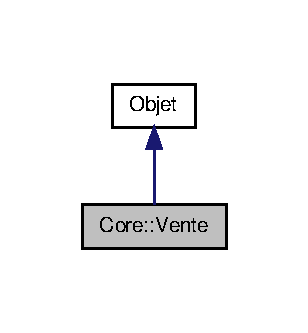
\includegraphics[width=148pt]{d5/da7/class_core_1_1_vente__inherit__graph}
\end{center}
\end{figure}


Graphe de collaboration de Core::Vente:\nopagebreak
\begin{figure}[H]
\begin{center}
\leavevmode
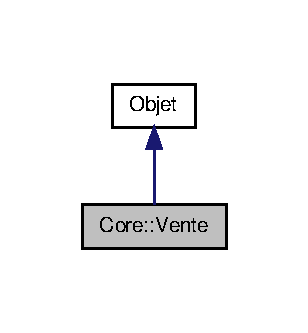
\includegraphics[width=148pt]{d6/d08/class_core_1_1_vente__coll__graph}
\end{center}
\end{figure}
\subsection*{Fonctions membres publiques}
\begin{DoxyCompactItemize}
\item 
\hypertarget{class_core_1_1_vente_a479f2669dd13f2eb62a543b874aef8b9}{
{\bfseries Vente} (QString code)}
\label{d9/d66/class_core_1_1_vente_a479f2669dd13f2eb62a543b874aef8b9}

\item 
\hypertarget{class_core_1_1_vente_a8ae390675f0c5beff6e7f74ff597af12}{
{\bfseries Vente} (QString code, double montant, QDate date)}
\label{d9/d66/class_core_1_1_vente_a8ae390675f0c5beff6e7f74ff597af12}

\item 
\hypertarget{class_core_1_1_vente_acc8ce82c4ed86bbcc0e7b187b497c3fd}{
QString {\bfseries getCode} () const }
\label{d9/d66/class_core_1_1_vente_acc8ce82c4ed86bbcc0e7b187b497c3fd}

\item 
\hypertarget{class_core_1_1_vente_a1b938be461750fcb6fa6b4b1630b623a}{
double {\bfseries getMontant} () const }
\label{d9/d66/class_core_1_1_vente_a1b938be461750fcb6fa6b4b1630b623a}

\item 
\hypertarget{class_core_1_1_vente_ab4498cdc8203b7c4fd1ae71730a0c014}{
QDate {\bfseries getDate} () const }
\label{d9/d66/class_core_1_1_vente_ab4498cdc8203b7c4fd1ae71730a0c014}

\item 
\hypertarget{class_core_1_1_vente_aaf0492f7bd78166842134da6c64fea4e}{
void {\bfseries setCode} (QString code)}
\label{d9/d66/class_core_1_1_vente_aaf0492f7bd78166842134da6c64fea4e}

\item 
\hypertarget{class_core_1_1_vente_a18eea1e317d5a2c203537a6fff850bdd}{
void {\bfseries setMontant} (double montant)}
\label{d9/d66/class_core_1_1_vente_a18eea1e317d5a2c203537a6fff850bdd}

\item 
\hypertarget{class_core_1_1_vente_a216e1d0533eb80d282a1b513e84aa3db}{
void {\bfseries setDate} (QDate date)}
\label{d9/d66/class_core_1_1_vente_a216e1d0533eb80d282a1b513e84aa3db}

\end{DoxyCompactItemize}
\subsection*{Propriétés}
\begin{DoxyCompactItemize}
\item 
\hypertarget{class_core_1_1_vente_abb1c7950bc7264a42cd4b7638218bd6d}{
QString {\bfseries code}}
\label{d9/d66/class_core_1_1_vente_abb1c7950bc7264a42cd4b7638218bd6d}

\item 
\hypertarget{class_core_1_1_vente_a01cf2b6d838af0908cd842651bc28cca}{
double {\bfseries montant}}
\label{d9/d66/class_core_1_1_vente_a01cf2b6d838af0908cd842651bc28cca}

\item 
\hypertarget{class_core_1_1_vente_a131c8a5328eeeb45a9274c27d6d573f9}{
QDate {\bfseries date}}
\label{d9/d66/class_core_1_1_vente_a131c8a5328eeeb45a9274c27d6d573f9}

\end{DoxyCompactItemize}


\subsection{Description détaillée}


Définition à la ligne 9 du fichier vente.h.



La documentation de cette classe a été générée à partir des fichiers suivants :\begin{DoxyCompactItemize}
\item 
core/vente.h\item 
core/vente.cpp\end{DoxyCompactItemize}

\printindex
\end{document}
